\documentclass[11pt,a4paper,oneside]{report}

% ============================================================
%  Γλώσσα και γραμματοσειρές
% ============================================================
\usepackage{polyglossia}
\setdefaultlanguage{greek}
\setotherlanguage{english}

\usepackage{fontspec}
\setmainfont{DejaVu Serif}[Scale=0.95]
\setsansfont{DejaVu Sans}[Scale=0.95]
\setmonofont{DejaVu Sans Mono}[Scale=0.88]
\newfontfamily\greekfonttt{DejaVu Sans Mono}[Scale=0.88]

% ============================================================
%  Διάταξη σελίδας και αποστάσεις
% ============================================================
\usepackage[a4paper,margin=2.5cm]{geometry}
\usepackage{setspace}
\onehalfspacing
\usepackage{microtype}
\usepackage{emptypage}
\usepackage{parskip}
\setlength{\parindent}{0pt}
\setlength{\parskip}{0.6em}

% ============================================================
%  Επικεφαλίδες κεφαλαίων
% ============================================================
\usepackage{titlesec}
\titleformat{\chapter}
  {\normalfont\LARGE\bfseries}{\chaptertitlename\ \thechapter.}{0.6em}{}
\titlespacing*{\chapter}{0pt}{50pt}{30pt}

% Πίνακας περιεχομένων: πρόθεμα «Κεφάλαιο X.»
\usepackage{tocloft}
\renewcommand{\cftchappresnum}{Κεφάλαιο\space}
\renewcommand{\cftchapaftersnum}{.}
\newlength{\mychapnumwidth}
\settowidth{\mychapnumwidth}{\bfseries Κεφάλαιο\space 99.\space}
\setlength{\cftchapnumwidth}{\mychapnumwidth}

% ============================================================
%  Μαθηματικά
% ============================================================
\usepackage{amsmath,amssymb,amsthm}
\usepackage{mathtools}

% Περιβάλλοντα θεωρημάτων
\newtheorem{theorem}{Θεώρημα}[chapter]
\newtheorem{lemma}[theorem]{Λήμμα}
\newtheorem{definition}[theorem]{Ορισμός}

% ============================================================
%  Παράθεση κώδικα (minted, απαιτεί --shell-escape)
% ============================================================
\usepackage[newfloat]{minted}
\usemintedstyle{friendly}
\setminted{
  fontsize=\small,
  frame=single,
  framesep=3mm,
  rulecolor=\color{gray!40},
  bgcolor=gray!7,
  linenos=false,
  breaklines=true,
  breakanywhere=true,
  xleftmargin=0pt,
  xrightmargin=0pt,
}
\usepackage{etoolbox}
\BeforeBeginEnvironment{minted}{\begin{minipage}{\linewidth}\vspace{0.4em}}
\AfterEndEnvironment{minted}{\end{minipage}\vspace{0.4em}}
\usepackage{caption}
\captionsetup[listing]{name=Κώδικας}

% ============================================================
%  Ψευδοκώδικας
% ============================================================
\usepackage[linesnumbered,ruled,vlined]{algorithm2e}
\SetKwInOut{Input}{Είσοδος}
\SetKwInOut{Output}{Έξοδος}
\SetKw{KwAnd}{\textbf{και}}
\SetKw{KwOr}{\textbf{ή}}
\SetKw{KwTrue}{\textbf{αληθές}}
\SetKw{KwFalse}{\textbf{ψευδές}}
\SetKwRepeat{Do}{επανάλαβε}{ενόσω}
\SetKwFor{While}{ενόσω}{επανάλαβε}{τέλος}
\SetKwFor{For}{για}{επανάλαβε}{τέλος}
\SetKwIF{If}{ElseIf}{Else}{αν}{τότε}{αλλιώς αν}{αλλιώς}{τέλος}
\SetKwFunction{FnContract}{ΣΥΜΠΤΥΞΗ}
\renewcommand{\algorithmcfname}{Αλγόριθμος}
\renewcommand{\algorithmautorefname}{Αλγόριθμος}

% ============================================================
%  Γραφικά, πίνακες, σύνδεσμοι
% ============================================================
\usepackage{graphicx}
\usepackage[section]{placeins}
\let\oldsubsection\subsection
\renewcommand{\subsection}{\FloatBarrier\oldsubsection}
\usepackage{tikz}
\usetikzlibrary{arrows.meta, positioning}
\usepackage{booktabs}
\usepackage{tabularx}
\usepackage{array}
\usepackage{xcolor}
\usepackage{enumitem}
\setlist{itemsep=2pt,parsep=2pt,topsep=3pt}

\usepackage{hyperref}
\hypersetup{
  colorlinks=true,
  linkcolor=black,
  urlcolor=blue!60!black,
  citecolor=black,
  pdftitle={Ένας ταχύτερος ισχυρά πολυωνυμικός αλγόριθμος για το πρόβλημα ροής ελαχίστου κόστους},
  pdfauthor={Diploma Thesis},
  bookmarksnumbered=true,
}

% ============================================================
%  Βοηθητικά
% ============================================================
\emergencystretch=2em
\tolerance=2000
\newcommand{\placeholder}[1]{%
  \begin{center}
  \textit{\color{gray!60!black}[PLACEHOLDER: #1]}
  \end{center}
}

% Αρίθμηση σελίδων
\usepackage{fancyhdr}
\usepackage{lastpage}
\pagestyle{fancy}
\fancyhf{}
\renewcommand{\headrulewidth}{0pt}
\renewcommand{\footrulewidth}{0pt}

% Εναλλαγή στυλ υποσέλιδου
\newcommand{\setfrontmatterfooter}{%
  \fancyhf{}%
  \renewcommand{\footrulewidth}{0pt}%
  \fancyfoot[C]{-- \thepage\ --}%
  \fancypagestyle{plain}{\fancyhf{}\renewcommand{\headrulewidth}{0pt}\renewcommand{\footrulewidth}{0pt}\fancyfoot[C]{-- \thepage\ --}}%
}
\newcommand{\setmainmatterfooter}{%
  \fancyhf{}%
  \renewcommand{\footrulewidth}{0.4pt}%
  \fancyfoot[R]{\thepage}%
  \fancypagestyle{plain}{\fancyhf{}\renewcommand{\headrulewidth}{0pt}\renewcommand{\footrulewidth}{0.4pt}\fancyfoot[R]{\thepage}}%
}

\begin{document}

% =============== ΕΞΩΦΥΛΛΟ ===============
\begin{titlepage}
\begin{tikzpicture}[remember picture, overlay]
  % Γαλάζια κάθετη λωρίδα
  \fill[color={rgb,255:red,146;green,205;blue,220}]
    ([xshift=0cm]current page.north west)
    rectangle
    ([xshift=1.4cm, yshift=7.5cm]current page.south west);
  % Λογότυπο τμήματος
  \node[anchor=south west, inner sep=0pt]
    at ([xshift=1.8cm, yshift=2.2cm]current page.south west)
    {
\includegraphics[width=2.8cm]{media/logo_cse_uoi.png}};
  % Όνομα τμήματος (ελληνικά)
  \node[anchor=south west, font=\bfseries\fontsize{11}{13}\selectfont]
    at ([xshift=5.0cm, yshift=4.2cm]current page.south west)
    {\begin{tabular}{@{}l@{}}
      ΤΜΗΜΑ ΜΗΧ.\ Η/Υ \& ΠΛΗΡΟΦΟΡΙΚΗΣ\\
      ΠΑΝΕΠΙΣΤΗΜΙΟ ΙΩΑΝΝΙΝΩΝ
    \end{tabular}};
  % Οριζόντια γραμμή διαχωρισμού
  \draw[black, line width=0.5pt]
    ([xshift=5.0cm, yshift=3.9cm]current page.south west) --
    ([xshift=-2.0cm, yshift=3.9cm]current page.south east);
  % Όνομα τμήματος (αγγλικά)
  \node[anchor=south west, font=\bfseries\fontsize{10}{12}\selectfont]
    at ([xshift=5.0cm, yshift=2.5cm]current page.south west)
    {\begin{english}\begin{tabular}{@{}l@{}}
      Department of Computer Science \& Engineering\\
      University of Ioannina
    \end{tabular}\end{english}};
\end{tikzpicture}

\centering
\vspace*{1.5cm}

{\Huge\bfseries Ένας ταχύτερος ισχυρά πολυωνυμικός αλγόριθμος\par}
\vspace{0.3cm}
{\Huge\bfseries για το πρόβλημα ροής ελαχίστου κόστους\par}

\vspace{2cm}
{\Large Νίκος Χατζηευφραιμίδης\par}

\vspace{2.5cm}
{\LARGE\bfseries Διπλωματική Εργασία\par}

\vspace{2cm}
{\large Επιβλέπων: Γεωργιάδης Λουκάς\par}

\vspace{2cm}
{\large Ιωάννινα, Μάιος 2026\par}

\end{titlepage}

\pagenumbering{roman}
\setfrontmatterfooter

% =============== ΕΥΧΑΡΙΣΤΙΕΣ ===============
\chapter*{Ευχαριστίες}
\addcontentsline{toc}{chapter}{Ευχαριστίες}

Θα ήθελα να ευχαριστήσω θερμά τον επιβλέποντα καθηγητή μου για την καθοδήγηση, τις εύστοχες παρατηρήσεις και την υπομονή του καθ' όλη τη διάρκεια εκπόνησης αυτής της διπλωματικής εργασίας. Οι συζητήσεις μας βοήθησαν καθοριστικά στο να κατανοήσω τις λεπτομέρειες του αλγορίθμου και να οργανώσω την υλοποίηση.

Ευχαριστώ επίσης τα μέλη της τριμελούς εξεταστικής επιτροπής για τον χρόνο και τα σχόλιά τους, καθώς και τους διδάσκοντες του προπτυχιακού προγράμματος σπουδών για τις γνώσεις που μου προσέφεραν σε όλα τα έτη της φοίτησής μου.

Τέλος, ευχαριστώ την οικογένεια και τους φίλους μου για τη στήριξη όλο αυτό το διάστημα.

% =============== ΠΕΡΙΛΗΨΗ ===============
\chapter*{Περίληψη}
\addcontentsline{toc}{chapter}{Περίληψη}

Η παρούσα διπλωματική εργασία μελετά τον αλγόριθμο του \textenglish{James~B.~Orlin} για την επίλυση του προβλήματος ροής ελαχίστου κόστους (\textenglish{minimum cost flow}) σε πολυωνυμικό και ισχυρά πολυωνυμικό χρόνο, όπως αυτός παρουσιάστηκε στην εργασία του 1993 στο περιοδικό \textenglish{Operations Research}. Η εργασία συνοδεύεται από υλοποίηση δύο εκδοχών του αλγορίθμου στη γλώσσα \textenglish{C}. Η πρώτη εκδοχή υλοποιεί την τεχνική κλιμάκωσης δεξιού μέλους (\textenglish{RHS-scaling}) των \textenglish{Edmonds} και \textenglish{Karp}, όπως περιγράφεται στην Ενότητα~3 του άρθρου. Η δεύτερη εκδοχή υλοποιεί τον πλήρη ισχυρά πολυωνυμικό αλγόριθμο της Ενότητας~4, ο οποίος προσθέτει στη βασική ιδέα την τεχνική της σύμπτυξης (\textenglish{contraction}) ισχυρά εφικτών ακμών, τη χαλαρωμένη επιλογή πηγής και καταβόθρας με παράμετρο $\alpha$, και το τελικό βήμα ανάκτησης βέλτιστης ροής μέσω υπολογισμού μέγιστης ροής στο υπο-δίκτυο μηδενικού μειωμένου κόστους.

Περιγράφεται λεπτομερώς η αρχιτεκτονική και η λογική κάθε υλοποίησης, ενώ παρέχεται και μια γεννήτρια τυχαίων ισορροπημένων δικτύων ροής σε \textenglish{Python}, η οποία χρησιμοποιεί τη βιβλιοθήκη \textenglish{NetworkX} και επιτρέπει τον συστηματικό έλεγχο ορθότητας των αλγορίθμων. Τέλος, παρουσιάζεται πειραματική αξιολόγηση των δύο εκδοχών και σύγκρισή τους με τη συνάρτηση υπολογισμού ροής ελαχίστου κόστους της \textenglish{NetworkX}, η οποία χρησιμοποιείται ως αναφορά ορθότητας.

\vspace{0.5em}
\textbf{Λέξεις κλειδιά:} ροή ελαχίστου κόστους, αλγόριθμος \textenglish{Orlin}, κλιμάκωση, \textenglish{RHS-scaling}, ισχυρά πολυωνυμικός αλγόριθμος, σύμπτυξη κόμβων, συντομότερα μονοπάτια, \textenglish{Dijkstra}, δίκτυα.

% =============== ABSTRACT ===============
\chapter*{\textenglish{Abstract}}
\addcontentsline{toc}{chapter}{Abstract}
\begin{english}
This thesis studies James~B.~Orlin's algorithm for solving the minimum cost flow problem in polynomial and strongly polynomial time, as presented in his 1993 Operations Research paper. The work is accompanied by an implementation of two versions of the algorithm in the C language. The first version implements the right-hand side scaling (RHS-scaling) technique of Edmonds and Karp, as described in Section~3 of the paper. The second version implements the full strongly polynomial algorithm of Section~4, which augments the basic idea with the contraction of strongly feasible arcs, a relaxed choice of source and sink controlled by a parameter $\alpha$, and a final step that recovers the optimal flow by computing a maximum flow on the subnetwork of arcs with zero reduced cost.

The architecture and logic of each implementation are described in detail, and a Python generator of random balanced flow networks is also provided; it uses the NetworkX library and enables systematic correctness checks of the algorithms. Finally, the two versions are evaluated experimentally and compared against the min cost flow routine of NetworkX, which is used as a correctness baseline.

\vspace{0.5em}
\textbf{Keywords:} minimum cost flow, Orlin's algorithm, scaling, RHS-scaling, strongly polynomial algorithm, node contraction, shortest paths, Dijkstra, networks.
\end{english}

% =============== ΠΕΡΙΕΧΟΜΕΝΑ ===============
\tableofcontents

\clearpage
\pagenumbering{arabic}
\setmainmatterfooter

% =============== ΚΕΦΑΛΑΙΑ ===============


\chapter{Εισαγωγή}

\section{Εισαγωγή}

Το πρόβλημα ροής ελαχίστου κόστους αποτελεί ένα από τα πιο θεμελιώδη προβλήματα στη θεωρία των δικτύων ροής. Δίνεται ένα κατευθυνόμενο δίκτυο στο οποίο κάθε κόμβος φέρει μια τιμή προσφοράς ή ζήτησης, κάθε ακμή φέρει ένα κόστος ανά μονάδα ροής και προαιρετικά μια άνω χωρητικότητα, και ζητείται να βρεθεί μια εφικτή ροή που ικανοποιεί τους περιορισμούς ισορροπίας μάζας σε κάθε κόμβο και ελαχιστοποιεί το συνολικό κόστος.

Το πρόβλημα αυτό έχει μελετηθεί εκτενώς λόγω της γενικότητάς του. Πολλά γνωστά προβλήματα συνδυαστικής βελτιστοποίησης, όπως το συντομότερο μονοπάτι, η μέγιστη ροή, η αντιστοίχιση σε διμερή γραφήματα και η κατανομή πόρων, αποτελούν ειδικές περιπτώσεις του. Για αυτόν τον λόγο, η αποδοτική επίλυσή του απασχόλησε τους ερευνητές για δεκαετίες και οδήγησε σε εκτεταμένη αλγοριθμική θεωρία.

Ένα από τα πιο σημαντικά επιτεύγματα στην ιστορία του προβλήματος είναι ο ισχυρά πολυωνυμικός αλγόριθμος του \textenglish{James~B.~Orlin}, ο οποίος δημοσιεύτηκε το 1993 στο περιοδικό \textenglish{Operations Research}. Ο αλγόριθμος βασίζεται σε μια βελτιωμένη εκδοχή της τεχνικής κλιμάκωσης δεξιού μέλους (\textenglish{right-hand side scaling}) των \textenglish{Edmonds} και \textenglish{Karp}, εμπλουτισμένη με την τεχνική της σύμπτυξης κόμβων. Επιλύει το μη χωρητικό πρόβλημα σε χρόνο ανάλογο με ένα πλήθος συντομότερων μονοπατιών που εξαρτάται μόνο από τον αριθμό κόμβων και ακμών, χωρίς εξάρτηση από τις αριθμητικές τιμές των κοστών ή των τιμών προσφοράς/ζήτησης.

Η παρούσα διπλωματική εργασία μελετά τον αλγόριθμο αυτόν και τον υλοποιεί σε δύο διακριτές εκδοχές σε γλώσσα \textenglish{C}. Η πρώτη εκδοχή υλοποιεί την απλή τεχνική κλιμάκωσης, η οποία εκτελείται σε πολυωνυμικό (αλλά όχι ισχυρά πολυωνυμικό) χρόνο. Η δεύτερη εκδοχή υλοποιεί ολόκληρο τον ισχυρά πολυωνυμικό αλγόριθμο, συμπεριλαμβανομένης της σύμπτυξης ισχυρά εφικτών ακμών, της αναίρεσης συμπτύξεων στο τέλος και του υπολογισμού βέλτιστης ροής μέσω μέγιστης ροής στο υπο-δίκτυο μηδενικού μειωμένου κόστους.

\section{Οργάνωση της διπλωματικής εργασίας}

Η εργασία οργανώνεται σε πέντε κεφάλαια, όπως περιγράφεται παρακάτω.

Στο Κεφάλαιο~1 παρουσιάζεται το αντικείμενο της εργασίας, η ιστορική εξέλιξη του προβλήματος, οι κυριότερες εφαρμογές του, οι βασικές θεωρητικές έννοιες που θα χρησιμοποιηθούν στη συνέχεια, καθώς και το προγραμματιστικό περιβάλλον της υλοποίησης.

Στο Κεφάλαιο~2 αναλύεται θεωρητικά ο αλγόριθμος του \textenglish{Orlin}. Περιγράφονται οι βασικοί ορισμοί, η έννοια της ψευδοροής και του υπολειπόμενου δικτύου, οι συνθήκες βελτιστότητας, η τεχνική κλιμάκωσης δεξιού μέλους και τα επιπλέον βήματα που απαιτούνται για την επέκταση σε ισχυρά πολυωνυμικό χρόνο.

Στο Κεφάλαιο~3 παρουσιάζεται αναλυτικά η υλοποίηση και των δύο εκδοχών του αλγορίθμου σε γλώσσα \textenglish{C}. Αναλύονται οι δομές δεδομένων, οι βασικές συναρτήσεις και οι λογικές επιλογές που έγιναν, καθώς και η γεννήτρια τυχαίων δικτύων σε \textenglish{Python} που χρησιμοποιήθηκε για την παραγωγή περιπτώσεων δοκιμής.

Στο Κεφάλαιο~4 παρουσιάζεται η πειραματική αξιολόγηση των δύο υλοποιήσεων. Συγκρίνονται ως προς την ορθότητα (χρησιμοποιώντας τη \textenglish{NetworkX} ως αναφορά) και ως προς την απόδοση σε διάφορα μεγέθη και πυκνότητες δικτύων.

Στο Κεφάλαιο~5 συνοψίζονται τα κύρια συμπεράσματα και προτείνονται πιθανές επεκτάσεις της εργασίας.

\section{Ιστορική αναδρομή}

Το πρόβλημα της ροής ελαχίστου κόστους έχει μακρά ιστορία, η οποία ξεκίνησε τη δεκαετία του 1960 με κλασικούς αλγορίθμους όπως η μέθοδος των \textenglish{Busacker} και \textenglish{Gowen}, οι οποίοι επαύξαναν τη ροή κατά μήκος συντομότερων μονοπατιών ως προς το κόστος, και η μέθοδος ακύρωσης κύκλων αρνητικού κόστους του \textenglish{Klein}. Οι πρώτες αυτές προσεγγίσεις, αν και ορθές, δεν ήταν πολυωνυμικές στον αυστηρό αριθμητικό περιορισμό του χρόνου.

Το καθοριστικό πρώτο βήμα στην κατεύθυνση πολυωνυμικών αλγορίθμων έγινε το 1972 από τους \textenglish{Jack Edmonds} και \textenglish{Richard Karp}, οι οποίοι εισήγαγαν την τεχνική κλιμάκωσης δεξιού μέλους (\textenglish{RHS-scaling}). Η τεχνική τους ανάγει το πρόβλημα σε μια ακολουθία λογαριθμικά πολλών φάσεων, σε καθεμία από τις οποίες επιλύονται λίγα προβλήματα συντομότερου μονοπατιού.

Το πιο σημαντικό θεωρητικό ερώτημα στον χώρο παρέμενε για χρόνια ανοιχτό: υπάρχει αλγόριθμος του οποίου ο χρόνος εκτέλεσης εξαρτάται μόνο από τις διαστάσεις του δικτύου και όχι από τις αριθμητικές τιμές των δεδομένων; Την καταφατική απάντηση έδωσε πρώτη η \textenglish{Éva Tardos} το 1985 με έναν ισχυρά πολυωνυμικό αλγόριθμο πολυπλοκότητας $O(m^4)$. Άλλοι ισχυρά πολυωνυμικοί αλγόριθμοι αναπτύχθηκαν από τους \textenglish{Orlin} (1984), \textenglish{Fujishige} (1986), \textenglish{Galil} και \textenglish{Tardos} (1986), καθώς και από τους \textenglish{Goldberg} και \textenglish{Tarjan} (1987, 1988).

Ο αλγόριθμος του \textenglish{Orlin} του 1993, τον οποίο μελετά αυτή η εργασία, βελτίωσε τον καλύτερο τότε χρόνο των \textenglish{Galil} και \textenglish{Tardos} κατά έναν παράγοντα $n^2/m$ και έδωσε έναν αλγόριθμο που επιλύει το μη χωρητικό πρόβλημα ως ακολουθία $O(n \log n)$ συντομότερων μονοπατιών. Με χρήση της υλοποίησης \textenglish{Fibonacci heap} του \textenglish{Dijkstra}, ο συνολικός χρόνος είναι $O\bigl(n \log n \,(m + n \log n)\bigr)$.

\section{Εφαρμογές του προβλήματος ροής ελαχίστου κόστους}

Το πρόβλημα της ροής ελαχίστου κόστους εμφανίζεται σε πλήθος πρακτικών εφαρμογών. Ενδεικτικά, μερικές κατηγορίες εφαρμογών παρουσιάζονται παρακάτω.

\textbf{Μεταφορές και \textenglish{logistics}.} Η κλασική περίπτωση είναι το πρόβλημα της μεταφοράς αγαθών από αποθήκες προς καταναλωτές με ελάχιστο κόστος μεταφοράς. Οι κόμβοι-αποθήκες έχουν θετική προσφορά, οι κόμβοι-αγορές έχουν ζήτηση, και τα κόστη των ακμών αντιπροσωπεύουν το κόστος αποστολής ανά μονάδα προϊόντος.

\textbf{Δίκτυα τηλεπικοινωνιών.} Η διανομή κίνησης μεταξύ κεντρικών κόμβων ενός δικτύου, όπου κάθε σύνδεση έχει χωρητικότητα και κόστος, μπορεί να μοντελοποιηθεί ως πρόβλημα ροής ελαχίστου κόστους. Το ίδιο ισχύει για τη δρομολόγηση πακέτων και τη διαχείριση εύρους ζώνης.

\textbf{Προγραμματισμός παραγωγής.} Προβλήματα επιλογής παραγωγικών γραμμών, αποθήκευσης προϊόντων στον χρόνο και ικανοποίησης περιοδικής ζήτησης αναδιαρθρώνονται συχνά ως ροές σε δίκτυα με δομή διαμερισμένη κατά χρονικά βήματα.

\textbf{Αντιστοίχιση σε διμερή γραφήματα.} Το πρόβλημα της τέλειας αντιστοίχισης ελαχίστου κόστους σε διμερές γράφημα είναι ειδική περίπτωση του προβλήματος ροής ελαχίστου κόστους και επιλύεται απευθείας από τους ίδιους αλγορίθμους.

\textbf{Υπολογιστική όραση.} Ορισμένα προβλήματα τμηματοποίησης εικόνας και αντιστοίχισης χαρακτηριστικών μεταξύ εικόνων αναδιαρθρώνονται ως προβλήματα ελαχίστου κόστους ροής.

\section{Θεωρητική Θεμελίωση}

Αυτή η ενότητα συνοψίζει τις θεμελιώδεις έννοιες της θεωρίας γραφημάτων και δικτύων ροής που χρησιμοποιούνται στη συνέχεια. Για περισσότερες λεπτομέρειες παραπέμπουμε στο εγχειρίδιο των \textenglish{Ahuja}, \textenglish{Magnanti} και \textenglish{Orlin}.

\begin{definition}[Κατευθυνόμενο γράφημα]
Κατευθυνόμενο γράφημα είναι ένα ζεύγος $G=(V,E)$, όπου $V$ είναι ένα πεπερασμένο σύνολο κόμβων και $E \subseteq V \times V$ είναι ένα σύνολο διατεταγμένων ζευγών κόμβων, που ονομάζονται ακμές. Για κάθε ακμή $(u,v)$, ο $u$ είναι η ουρά και ο $v$ η κεφαλή της ακμής.
\end{definition}

\begin{definition}[Δίκτυο ροής]
Δίκτυο ροής είναι ένα κατευθυνόμενο γράφημα $G=(V,E)$ εφοδιασμένο με:
\begin{itemize}
  \item συνάρτηση κόστους $c: E \to \mathbb{Z}$ που αντιστοιχίζει σε κάθε ακμή ένα ακέραιο κόστος ανά μονάδα ροής·
  \item συνάρτηση προσφοράς/ζήτησης $b: V \to \mathbb{Z}$, όπου $b(v)>0$ σημαίνει ότι ο κόμβος $v$ προσφέρει $b(v)$ μονάδες, $b(v)<0$ σημαίνει ότι ο κόμβος απορροφά $|b(v)|$ μονάδες, και $b(v)=0$ αντιστοιχεί σε κόμβο διαμεταγωγής·
  \item προαιρετικά, συνάρτηση χωρητικότητας $u: E \to \mathbb{Z}_{+} \cup \{\infty\}$ που θέτει άνω όριο ροής.
\end{itemize}
\end{definition}

\begin{definition}[Ροή]
Ροή είναι συνάρτηση $x: E \to \mathbb{R}_{+}$ που σε κάθε ακμή $(i,j)$ αποδίδει μια μη αρνητική τιμή $x_{ij}$. Η ροή ονομάζεται \emph{εφικτή} αν ικανοποιεί τους περιορισμούς ισορροπίας μάζας σε κάθε κόμβο:
\[
\sum_{j:(i,j)\in E} x_{ij} \;-\; \sum_{j:(j,i)\in E} x_{ji} \;=\; b(i), \qquad \forall\, i \in V.
\]
\end{definition}

\begin{definition}[Ψευδοροή]
Ψευδοροή είναι μια συνάρτηση $x: E \to \mathbb{R}_{+}$ που ικανοποιεί μόνο τους περιορισμούς μη αρνητικότητας, αλλά επιτρέπεται να παραβιάζει τους περιορισμούς ισορροπίας μάζας. Για δοθείσα ψευδοροή $x$, το \emph{πλεόνασμα} ή \emph{\textenglish{imbalance}} του κόμβου $i$ ορίζεται ως
\[
e(i) \;=\; b(i) \;+\; \sum_{j:(j,i)\in E} x_{ji} \;-\; \sum_{j:(i,j)\in E} x_{ij}.
\]
Αν $e(i) > 0$, ο $i$ λέγεται \emph{πηγή}· αν $e(i) < 0$, λέγεται \emph{καταβόθρα}· αν $e(i) = 0$, λέγεται \emph{ισορροπημένος}.
\end{definition}

\begin{definition}[Υπολειπόμενο δίκτυο]
Για δοθείσα ψευδοροή $x$, το υπολειπόμενο δίκτυο $G(x)$ προκύπτει από το $G$ με τον εξής τρόπο: κάθε ακμή $(i,j) \in E$ του αρχικού αντικαθίσταται από δύο ακμές, την \emph{προσθετική} $(i,j)$ με κόστος $c_{ij}$ και άπειρη υπολειπόμενη χωρητικότητα (στην μη χωρητική περίπτωση) και την \emph{αφαιρετική} $(j,i)$ με κόστος $-c_{ij}$ και υπολειπόμενη χωρητικότητα ίση με την τρέχουσα ροή $x_{ij}$. Στο υπολειπόμενο δίκτυο διατηρούμε μόνο ακμές με θετική υπολειπόμενη χωρητικότητα.
\end{definition}

\begin{definition}[Δυναμικά κόμβων και μειωμένο κόστος]
Σε κάθε κόμβο $i$ αντιστοιχούμε μια δυική μεταβλητή $\pi(i)$ που ονομάζεται \emph{δυναμικό}. Το \emph{μειωμένο κόστος} μιας ακμής $(i,j)$ ως προς τα δυναμικά $\pi$ ορίζεται ως
\[
c^{\pi}_{ij} \;=\; c_{ij} - \pi(i) + \pi(j).
\]
\end{definition}

\section{Εισαγωγή στο πρόβλημα ροής ελαχίστου κόστους}

Το μη χωρητικό πρόβλημα ροής ελαχίστου κόστους διατυπώνεται ως το παρακάτω πρόβλημα γραμμικού προγραμματισμού:
\begin{align*}
\text{ελαχιστοποίηση}\quad & \sum_{(i,j)\in E} c_{ij}\, x_{ij} \\
\text{υπό}\quad & \sum_{j:(i,j)\in E} x_{ij} \;-\; \sum_{j:(j,i)\in E} x_{ji} \;=\; b(i), \quad \forall\, i \in V \\
& x_{ij} \;\geq\; 0, \quad \forall\, (i,j) \in E.
\end{align*}

Θα υποθέσουμε στη συνέχεια, ακολουθώντας τη σύμβαση του \textenglish{Orlin}, ότι το δίκτυο είναι ισχυρά συνδεδεμένο και ότι όλα τα κόστη είναι μη αρνητικά. Οι δύο αυτές παραδοχές δεν αποτελούν περιορισμό, καθώς μπορούν να ικανοποιηθούν με κλασικούς μετασχηματισμούς (προσθήκη τεχνητού κόμβου με τεχνητές ακμές μεγάλου κόστους για ισχυρή συνδεδεμένη, αλλαγή κόστους μέσω δυναμικών για μη αρνητικότητα).

Το πρόβλημα διαθέτει μια κλασική δυική διατύπωση. Σε κάθε περιορισμό ισορροπίας μάζας αντιστοιχούμε μια δυική μεταβλητή $\pi(i)$. Τότε το δυικό πρόβλημα έχει τη μορφή:
\begin{align*}
\text{μεγιστοποίηση}\quad & \sum_{i\in V} b(i)\, \pi(i) \\
\text{υπό}\quad & \pi(i) - \pi(j) \;\leq\; c_{ij}, \quad \forall\, (i,j) \in E.
\end{align*}

\section{Συνθήκες βελτιστότητας και δυϊκό πρόβλημα}

Οι συνθήκες συμπληρωματικής χαλαρότητας για το πρωτεύον-δυικό ζεύγος παίρνουν την εξής μορφή. Χρησιμοποιώντας τα μειωμένα κόστη $c^{\pi}_{ij} = c_{ij} - \pi(i) + \pi(j)$, οι συνθήκες βελτιστότητας εκφράζονται στο υπολειπόμενο δίκτυο ως εξής:

Μια ροή $x$ είναι βέλτιστη αν και μόνο αν υπάρχει διάνυσμα δυναμικών $\pi$ τέτοιο ώστε όλες οι ακμές του υπολειπόμενου δικτύου $G(x)$ να έχουν μη αρνητικό μειωμένο κόστος, δηλαδή
\[
c^{\pi}_{ij} \;\geq\; 0, \qquad \forall\, (i,j) \in E(G(x)).
\]

Η ισοδυναμία αυτή έχει θεμελιώδεις συνέπειες για τον σχεδιασμό αλγορίθμων. Αν μια τρέχουσα ψευδοροή $x$ και τρέχοντα δυναμικά $\pi$ ικανοποιούν την παραπάνω συνθήκη, τότε κάθε βελτίωση της ροής μπορεί να γίνει μόνο κατά μήκος μονοπατιών μηδενικού μειωμένου κόστους, ή ακόμα πιο αποδοτικά, κατά μήκος συντομότερων μονοπατιών ως προς μειωμένα κόστη από μια πηγή σε μια καταβόθρα. Ένα βασικό λήμμα (Λήμμα~3 του άρθρου) εγγυάται ότι, αν αντικαταστήσουμε τα δυναμικά ως $\pi := \pi - d$, όπου $d$ είναι οι αποστάσεις συντομότερου μονοπατιού ως προς τα μειωμένα κόστη, τα νέα δυναμικά διατηρούν τη συνθήκη βελτιστότητας και επιπλέον οι ακμές του συντομότερου μονοπατιού αποκτούν μηδενικό μειωμένο κόστος, οπότε η επαύξηση κατά μήκος του μονοπατιού είναι ασφαλής.

\section{Επισκόπηση αλγορίθμων για το πρόβλημα ροής ελαχίστου κόστους}

Η έρευνα στον χώρο των αλγορίθμων για το πρόβλημα ροής ελαχίστου κόστους χωρίζεται σε δύο μεγάλες κατηγορίες. Η πρώτη αφορά πολυωνυμικούς αλγορίθμους που εξαρτώνται από τις αριθμητικές τιμές του δικτύου μέσω λογαριθμικών όρων (π.χ.\ $\log C$ για ακέραια κόστη με μέγιστη απόλυτη τιμή $C$). Η δεύτερη αφορά ισχυρά πολυωνυμικούς αλγορίθμους, των οποίων ο χρόνος εκτέλεσης εκφράζεται αποκλειστικά μέσω του $n$ και του $m$.

Στην πρώτη κατηγορία ανήκουν οι αλγόριθμοι κλιμάκωσης των \textenglish{Edmonds} και \textenglish{Karp} (1972) και του \textenglish{Röck} (1980), οι αλγόριθμοι διπλής κλιμάκωσης των \textenglish{Ahuja}, \textenglish{Goldberg}, \textenglish{Orlin} και \textenglish{Tarjan} (1988), καθώς και ο αλγόριθμος διαδοχικής προσέγγισης των \textenglish{Goldberg} και \textenglish{Tarjan} (1987). Στη δεύτερη κατηγορία ανήκουν οι αλγόριθμοι της \textenglish{Tardos} (1985), του \textenglish{Fujishige} (1986), των \textenglish{Galil} και \textenglish{Tardos} (1986), καθώς και ο αλγόριθμος του \textenglish{Orlin} (1993).

Για τη σύγκριση των αλγορίθμων αυτών παραπέμπουμε στον πίνακα της Εικόνας~1 του άρθρου του \textenglish{Orlin}, ο οποίος συνοψίζει τη ροή εξελίξεων. Στην παρούσα εργασία μας ενδιαφέρει κυρίως η σύγκριση του βασικού αλγορίθμου κλιμάκωσης των \textenglish{Edmonds-Karp} (την εκδοχή που υλοποιεί η Ενότητα~3 του άρθρου) με τον ισχυρά πολυωνυμικό αλγόριθμο του \textenglish{Orlin} (Ενότητα~4).

\section{Πολυπλοκότητα αλγορίθμων}

Η χρονική πολυπλοκότητα ενός αλγορίθμου εκφράζεται συνήθως ως συνάρτηση του μεγέθους της εισόδου, όπου ως μέγεθος εννοούμε συνήθως το πλήθος κόμβων $n$ και ακμών $m$ ενός δικτύου. Στον χώρο των αλγορίθμων δικτύων ροής, είναι κλασικό να εκφράζουμε τους χρόνους ως γινόμενα του τύπου [αριθμός επαναλήψεων]~$\times$~[χρόνος επαναληπτικού βήματος].

Ο αλγόριθμος της Ενότητας~3 του \textenglish{Orlin} επιλύει το μη χωρητικό πρόβλημα σε $O(n\log U)$ συντομότερα μονοπάτια, όπου $U$ η μέγιστη απόλυτη τιμή της προσφοράς/ζήτησης. Ο αλγόριθμος της Ενότητας~4 τα επιλύει σε $O(n \log n)$ συντομότερα μονοπάτια, χωρίς εξάρτηση από τις αριθμητικές τιμές.

Στην υλοποίησή μας χρησιμοποιούμε την απλή υλοποίηση του \textenglish{Dijkstra} με αναζήτηση γραμμικού χρόνου της ελάχιστης απόστασης, οπότε κάθε κλήση συντομότερου μονοπατιού τρέχει σε $O(nm)$ χρόνο. Αυτό απλοποιεί τον κώδικα αλλά δίνει ένα χειρότερο άνω όριο από το θεωρητικά βέλτιστο που πετυχαίνεται με \textenglish{Fibonacci heaps}. Επιλέξαμε αυτήν την προσέγγιση γιατί επικεντρωνόμαστε στη σωστή ενσάρκωση της αλγοριθμικής δομής του \textenglish{Orlin}, όχι στη βέλτιστη εκμετάλλευση δομών δεδομένων για τον \textenglish{Dijkstra}.

\section{Προγραμματιστικό περιβάλλον και εργαλεία}

Η υλοποίηση του αλγορίθμου έγινε σε γλώσσα \textenglish{C}. Η επιλογή της \textenglish{C} έγινε κυρίως για λόγους απόδοσης και διαφάνειας στη διαχείριση μνήμης: όλες οι δομές δεδομένων δηλώνονται ρητά, όλες οι εκχωρήσεις γίνονται χειροκίνητα και η δομή του κώδικα αντιστοιχεί πιστά στα βήματα του αλγορίθμου όπως περιγράφονται στο άρθρο.

Ο κώδικας μεταγλωττίζεται με τον μεταγλωττιστή \texttt{gcc}. Το \texttt{Makefile} που συνοδεύει την εργασία ορίζει δύο στόχους:
\begin{itemize}
  \item \texttt{mcf\_section3}: υλοποιεί την τεχνική κλιμάκωσης των \textenglish{Edmonds-Karp} (Ενότητα~3 του άρθρου).
  \item \texttt{mcf\_section4}: υλοποιεί τον ισχυρά πολυωνυμικό αλγόριθμο (Ενότητα~4 του άρθρου).
\end{itemize}
Οι σημαίες μεταγλώττισης που χρησιμοποιούνται είναι \texttt{-Wall -Wextra -g}, οι οποίες ενεργοποιούν όλες τις προειδοποιήσεις και συμπεριλαμβάνουν πληροφορίες εκσφαλμάτωσης.

Για τη δημιουργία τυχαίων δικτύων δοκιμής χρησιμοποιείται ένα σενάριο \textenglish{Python} (\texttt{generator.py}) που αξιοποιεί τη βιβλιοθήκη \textenglish{NetworkX}. Η \textenglish{NetworkX} προσφέρει εύκολη κατασκευή κατευθυνόμενων γραφημάτων, ελέγχους ισχυρής συνδεδεμένης και, σημαντικό για την εργασία μας, ενσωματωμένη υλοποίηση επιλύτη ροής ελαχίστου κόστους (συνάρτηση \texttt{min\_cost\_flow\_cost}), την οποία χρησιμοποιούμε ως αναφορά ορθότητας. Η γεννήτρια υποστηρίζει παράμετρο \texttt{seed} για αναπαραγωγιμότητα των πειραμάτων.

Η μορφή αρχείου εισόδου που υποστηρίζουν και οι δύο υλοποιήσεις είναι η εξής: η πρώτη γραμμή περιέχει δύο ακεραίους, $n$ και $m$, τον αριθμό κόμβων και ακμών αντίστοιχα. Η δεύτερη γραμμή περιέχει $n$ ακεραίους χωρισμένους με κενό, τις τιμές $b(i)$ για κάθε κόμβο. Ακολουθούν $m$ γραμμές, καθεμία στη μορφή \texttt{from to cost}, που περιγράφουν τις ακμές.

\chapter{Ο αλγόριθμος του \textenglish{Orlin} (1993)}

\section{Συμβολισμός και ορισμοί}

Θεωρούμε κατευθυνόμενο δίκτυο $G=(V,E)$ με $|V|=n$ και $|E|=m$. Σε κάθε ακμή $(i,j) \in E$ αντιστοιχίζεται ακέραιο κόστος $c_{ij} \geq 0$. Σε κάθε κόμβο $i$ αντιστοιχίζεται ακέραιος αριθμός $b(i)$, που δηλώνει την προσφορά (αν θετικός) ή τη ζήτηση (αν αρνητικός) του κόμβου. Θέτουμε $U = \max_{i} |b(i)|$.

Η ροή σημειώνεται $x = (x_{ij})$ και αποτελεί διάνυσμα επί των ακμών. Δεδομένης ροής $x$, το πλεόνασμα του κόμβου $i$ είναι
\[
e(i) \;=\; b(i) + \sum_{(j,i)\in E} x_{ji} - \sum_{(i,j)\in E} x_{ij}.
\]
Σημειώνουμε ως
\[
S(\Delta) = \{\, i \in V : e(i) \geq \Delta \,\}, \qquad T(\Delta) = \{\, i \in V : e(i) \leq -\Delta \,\}
\]
τα σύνολα κόμβων με πλεόνασμα ή έλλειμμα τουλάχιστον $\Delta$, αντίστοιχα.

Σε κάθε κόμβο αντιστοιχίζεται δυναμικό $\pi(i) \in \mathbb{R}$. Το μειωμένο κόστος μιας ακμής $(i,j)$ είναι $c^{\pi}_{ij} = c_{ij} - \pi(i) + \pi(j)$. Το υπολειπόμενο δίκτυο $G(x)$ περιέχει, για κάθε ακμή $(i,j) \in E$, την προσθετική ακμή $(i,j)$ με κόστος $c_{ij}$ και άπειρη υπολειπόμενη χωρητικότητα, και την αφαιρετική ακμή $(j,i)$ με κόστος $-c_{ij}$ και υπολειπόμενη χωρητικότητα $x_{ij}$ (η οποία υπάρχει μόνο αν $x_{ij} > 0$).

\section{Ψευδοροή και υπολειπόμενο δίκτυο}

Η έννοια της ψευδοροής είναι κεντρική στον αλγόριθμο του \textenglish{Orlin}. Αντί να διατηρούμε σε κάθε βήμα μια εφικτή ροή και να την βελτιώνουμε, διατηρούμε μια ψευδοροή (η οποία ενδέχεται να παραβιάζει την ισορροπία σε ορισμένους κόμβους) και προσπαθούμε να την κάνουμε εφικτή. Τα πλεονάσματα $e(i)$ παρακολουθούν αυτή τη διαφορά από την ισορροπία.

Η κεντρική λειτουργία είναι η επαύξηση κατά μήκος μονοπατιού από πηγή προς καταβόθρα. Αν ο $s$ είναι κόμβος με $e(s) \geq \Delta$ και ο $t$ είναι κόμβος με $e(t) \leq -\Delta$, και υπάρχει μονοπάτι $P$ στο $G(x)$ από τον $s$ στον $t$, τότε μπορούμε να στείλουμε $\Delta$ μονάδες ροής κατά μήκος του $P$. Αυτό μειώνει το $e(s)$ κατά $\Delta$ και αυξάνει το $e(t)$ κατά $\Delta$, ενώ ενημερώνει τις υπολειπόμενες χωρητικότητες του μονοπατιού.

Για να αποφύγουμε την αναζήτηση κύκλων αρνητικού μειωμένου κόστους, επιλέγουμε πάντοτε το συντομότερο μονοπάτι από τον $s$ στον $t$ ως προς τα μειωμένα κόστη. Το παρακάτω λήμμα (Λήμμα~3 στο άρθρο του \textenglish{Orlin}) διασφαλίζει ότι αυτή η επιλογή διατηρεί τη συνθήκη βελτιστότητας.

\section{Δυναμικά κόμβων και μειωμένα κόστη}

\begin{lemma}[Ενημέρωση δυναμικών]
Έστω ψευδοροή $x$ που ικανοποιεί τη συνθήκη βελτιστότητας ως προς δυναμικά $\pi$, και έστω $d(i)$ η απόσταση συντομότερου μονοπατιού από τον κόμβο-πηγή $s$ σε κάθε κόμβο $i$ στο $G(x)$, χρησιμοποιώντας μειωμένα κόστη $c^{\pi}$ ως μήκη ακμών. Θέτουμε $\pi' = \pi - d$. Τότε:
\begin{enumerate}
  \item Η ψευδοροή $x$ ικανοποιεί τη συνθήκη βελτιστότητας και ως προς τα $\pi'$.
  \item Για κάθε ακμή $(i,j)$ επί ενός συντομότερου μονοπατιού από τον $s$, το μειωμένο κόστος ως προς τα $\pi'$ είναι μηδέν.
\end{enumerate}
\end{lemma}

Η ιδιότητα αυτή είναι καθοριστική: ύστερα από επαύξηση κατά μήκος του συντομότερου μονοπατιού, οι νέες αφαιρετικές ακμές που εμφανίζονται στο υπολειπόμενο δίκτυο έχουν επίσης μηδενικό μειωμένο κόστος (αρνητικό του μηδενικού, δηλαδή πάλι μηδέν), οπότε η συνθήκη βελτιστότητας συνεχίζει να ισχύει.

\section{Η τεχνική κλιμάκωσης των \textenglish{Edmonds-Karp} (\textenglish{RHS-Scaling})}

\subsection{Φάσεις κλιμάκωσης}

Η τεχνική της κλιμάκωσης δεξιού μέλους επιλύει το πρόβλημα ως μια ακολουθία φάσεων, καθεμία από τις οποίες αντιστοιχεί σε μια τιμή κλίμακας $\Delta$. Αρχικά θέτουμε $\Delta = 2^{\lceil \log U \rceil}$. Σε κάθε φάση, η τιμή $\Delta$ μειώνεται στο μισό. Σε κάθε φάση εξετάζουμε τα σύνολα $S(\Delta)$ και $T(\Delta)$ και, όσο υπάρχει κόμβος σε κάθε ένα, εκτελούμε επαύξηση κατά μήκος συντομότερου μονοπατιού που στέλνει $\Delta$ μονάδες.

Ένα κλειδί είναι ότι κάθε φάση απαιτεί μόνο λίγες επαυξήσεις. Στην αρχή κάθε φάσης ισχύει ότι $S(2\Delta) = \emptyset$ ή $T(2\Delta) = \emptyset$. Στην πρώτη περίπτωση, κάθε επαύξηση αφαιρεί έναν κόμβο από το $S(\Delta)$· στη δεύτερη, αφαιρεί έναν κόμβο από το $T(\Delta)$. Έτσι το Λήμμα~6 του άρθρου δίνει ότι ο αριθμός επαυξήσεων σε μια φάση δεν ξεπερνά τον αριθμό κόμβων που αναγεννώνται στην αρχή της φάσης. Συνεπώς, το συνολικό πλήθος επαυξήσεων είναι $O(n \log U)$.

\subsection{Επαυξήσεις κατά μήκος συντομότερων μονοπατιών}

Το κρίσιμο λήμμα (Λήμμα~5 του άρθρου) εγγυάται ότι, σε κάθε σημείο του αλγορίθμου, κάθε ροή ή υπολειπόμενη χωρητικότητα είναι ακέραιο πολλαπλάσιο του τρέχοντος $\Delta$. Αυτό εξασφαλίζει ότι μπορούμε πάντοτε να στέλνουμε ολόκληρα $\Delta$ μονάδων κατά μήκος οποιουδήποτε μονοπατιού με θετική υπολειπόμενη χωρητικότητα.

\begin{algorithm}[H]
\caption{\textenglish{RHS-Scaling} (Εικόνα~3 του άρθρου του \textenglish{Orlin})}
\Input{Δίκτυο $G=(V,E)$ με κόστη $c$ και τιμές $b(\cdot)$}
\Output{Βέλτιστη ροή $x$ και δυναμικά $\pi$}
$x \leftarrow 0$\;
$\pi \leftarrow 0$\;
$e \leftarrow b$\;
$U \leftarrow \max\{\,|b(i)| : i \in V\,\}$\;
$\Delta \leftarrow 2^{\lceil \log U \rceil}$\;
\While{υπάρχει $i$ με $e(i) \neq 0$}{
  \tcc{$\Delta$-φάση κλιμάκωσης}
  $S(\Delta) \leftarrow \{\, i : e(i) \geq \Delta \,\}$\;
  $T(\Delta) \leftarrow \{\, i : e(i) \leq -\Delta \,\}$\;
  \While{$S(\Delta) \neq \emptyset$ \KwAnd $T(\Delta) \neq \emptyset$}{
    επέλεξε $k \in S(\Delta)$ και $v \in T(\Delta)$\;
    υπολόγισε αποστάσεις $d(i)$ από τον $k$ στο $G(x)$ με μήκη $c^{\pi}$\;
    $\pi(i) \leftarrow \pi(i) - d(i),\ \forall\, i \in V$\;
    επαύξησε $\Delta$ μονάδες κατά μήκος του συντομότερου μονοπατιού $k \to v$\;
    ενημέρωσε $x,\, e,\, S(\Delta),\, T(\Delta)$\;
  }
  $\Delta \leftarrow \Delta / 2$\;
}
\end{algorithm}

\subsection{Ορθότητα και πολυπλοκότητα}

Η ορθότητα προκύπτει από τον συνδυασμό τριών παρατηρήσεων. Πρώτον, η αρχικοποίηση ($x = 0$, $\pi = 0$) ικανοποιεί τη συνθήκη βελτιστότητας, καθώς όλες οι ακμές του υπολειπόμενου δικτύου έχουν μη αρνητικό κόστος. Δεύτερον, κάθε επαύξηση με ενημέρωση δυναμικών διατηρεί τη συνθήκη βελτιστότητας. Τρίτον, όταν $\Delta < 1$ και όλοι οι ακέραιοι αρχικοί αριθμοί έχουν εξαντλήσει τις κλίμακες, η ακεραιότητα εξασφαλίζει ότι όλα τα πλεονάσματα έχουν μηδενιστεί, άρα η ψευδοροή είναι πλέον εφικτή ροή.

Η συνολική πολυπλοκότητα του \textenglish{RHS-Scaling} για το μη χωρητικό πρόβλημα είναι $O(n\log U)$ συντομότερα μονοπάτια. Αν σημειώσουμε $S(n,m)$ τον χρόνο υπολογισμού ενός συντομότερου μονοπατιού σε γράφημα με $n$ κόμβους και $m$ ακμές με μη αρνητικά κόστη, ο συνολικός χρόνος γίνεται $O\bigl(n\log U \cdot S(n,m)\bigr)$.

\section{Από τον \textenglish{RHS-Scaling} στον ισχυρά πολυωνυμικό αλγόριθμο}

Η κεντρική ιδέα του \textenglish{Orlin} (1993) είναι η δυνατότητα να αντικατασταθεί ο παράγοντας $\log U$ με παράγοντα $\log n$, κάτι που οδηγεί σε αλγόριθμο του οποίου ο χρόνος δεν εξαρτάται από τις αριθμητικές τιμές της εισόδου.

Για να το πετύχει αυτό, ο αλγόριθμος εισάγει τρεις ιδέες: (α) την έννοια της ισχυρά εφικτής ακμής και τη σύμπτυξη, (β) μια τροποποίηση της επιλογής πηγής και καταβόθρας μέσω μιας παραμέτρου $\alpha \in (1/2,\, 1)$, και (γ) έναν μηχανισμό πλήρους αναγέννησης που επαναφέρει το $\Delta$ στη μέγιστη τρέχουσα τιμή πλεονάσματος όταν οι ροές μηδενίζονται.

\subsection{Η έννοια της σύμπτυξης}

Η βασική διαίσθηση είναι η εξής. Αν σε μια χρονική στιγμή διαπιστώσουμε ότι η ροή μιας ακμής είναι αρκετά μεγάλη ώστε να αποκλειστεί η περίπτωση να μηδενιστεί σε κάποια επόμενη φάση, τότε γνωρίζουμε ότι αυτή η ακμή θα έχει θετική ροή στη βέλτιστη λύση. Από τις συνθήκες συμπληρωματικής χαλαρότητας έπεται ότι το βέλτιστο μειωμένο κόστος αυτής της ακμής είναι μηδέν. Αν μετασχηματίσουμε τα κόστη του δικτύου σε μειωμένα κόστη, η ακμή αποκτά μηδενικό κόστος και τα βέλτιστα δυναμικά των δύο άκρων της γίνονται ίσα.

Αυτή η ισοδυναμία επιτρέπει τη σύμπτυξη των δύο άκρων σε έναν κόμβο: το δίκτυο μικραίνει κατά έναν κόμβο, και το νέο δίκτυο έχει ως λύση ουσιαστικά την ίδια βέλτιστη ροή. Επειδή οι συμπτύξεις είναι το πολύ $n-1$, η συνολική μείωση μεγέθους οδηγεί σε ανάλογη μείωση στον αριθμό φάσεων.

\subsection{Ισχυρά εφικτές ακμές}

Για να εκφραστεί τυπικά η παραπάνω διαίσθηση, ο \textenglish{Orlin} εισάγει στην Ενότητα~4.1 του άρθρου την έννοια της \emph{ισχυρά εφικτής ακμής}: μια ακμή $(i,j)$ ονομάζεται ισχυρά εφικτή στη $\Delta$-φάση αν η ροή της ξεπερνά το $2n\Delta$. Στον ίδιο τον αλγόριθμο, ωστόσο, η σύμπτυξη ενεργοποιείται μόνο όταν η ροή φτάσει το αυστηρότερο όριο $3n\Delta$, ώστε να συνυπολογιστούν και οι έως $n-1$ επιπλέον επαυξήσεις που προκαλούν οι ίδιες οι συμπτύξεις. Όταν μια ακμή ικανοποιήσει αυτό το κατώφλι, συμπτύσσονται τα άκρα της.

Το Λήμμα~11 του άρθρου εγγυάται ότι, αν $x_{ij} \geq 3n\Delta$ σε μια $\Delta$-φάση, τότε $x_{ij} > 0$ σε όλες τις μετέπειτα φάσεις. Ο αλγόριθμος λοιπόν, στην αρχή κάθε φάσης, ελέγχει αν υπάρχουν τέτοιες ακμές και, αν υπάρχουν, προχωρά σε συμπτύξεις.

\subsection{Ένα παθολογικό παράδειγμα}

Ωστόσο, η αφελής εφαρμογή του \textenglish{RHS-Scaling} με συμπτύξεις δεν δίνει αμέσως ισχυρά πολυωνυμικό αλγόριθμο. Το άρθρο παρουσιάζει στην Ενότητα~4.2 ένα παθολογικό παράδειγμα (Εικόνα~4 του άρθρου): ένα δίκτυο τεσσάρων κόμβων με προσφορές/ζητήσεις που εξαρτώνται από μια μεγάλη παράμετρο $M$. Σε αυτό το δίκτυο, η τυπική συμπτυκτική διαδικασία δημιουργεί έναν κόμβο με εξαιρετικά μικρή προσφορά/ζήτηση αλλά με πλεόνασμα συγκρίσιμο με το $\Delta$, γεγονός που τον αναγκάζει να αναγεννάται σε πολλές φάσεις και τελικά εκθέτει τον αλγόριθμο σε $\log M$ φάσεις.

Αυτή η παρατήρηση οδηγεί στην τροποποίηση της επιλογής πηγής και καταβόθρας που περιγράφεται στην επόμενη υποενότητα.

\subsection{Τροποποίηση των κανόνων επαύξησης}

Η τροποποίηση είναι απλή αλλά κρίσιμη: αντί να αναζητούμε κόμβους με $e(i) \geq \Delta$ και $e(i) \leq -\Delta$, αναζητούμε κόμβους με $e(i) \geq \alpha\Delta$ και $e(i) \leq -\alpha\Delta$, για μια επιλεγμένη παράμετρο $\alpha \in (1/2,\, 1)$. Η επιλογή αυτή εξασφαλίζει ότι κάθε αναγεννημένος κόμβος έχει πλεόνασμα πολύ κοντά σε $\alpha\Delta$, όχι οριακά κοντά στο $\Delta$, γεγονός που σπάει το παθολογικό σενάριο.

Η υλοποίησή μας χρησιμοποιεί $\alpha = 3/4$, εκφρασμένο ως κλάσμα ώστε να αποφεύγονται οι αριθμητικές πράξεις κινητής υποδιαστολής. Συγκεκριμένα, ένας κόμβος $i$ είναι πηγή αν $4 \cdot e(i) \geq 3 \cdot \Delta$ και είναι καταβόθρα αν $4 \cdot e(i) \leq -3 \cdot \Delta$.

\section{Ο ισχυρά πολυωνυμικός αλγόριθμος}

\subsection{Περιγραφή αλγορίθμου}

Ο ισχυρά πολυωνυμικός αλγόριθμος του \textenglish{Orlin} (Εικόνα~5 του άρθρου) μπορεί να περιγραφεί ως εξής:

\begin{algorithm}[H]
\caption{\textenglish{Strongly-Polynomial} (Εικόνα~5 του άρθρου του \textenglish{Orlin})}
\Input{Δίκτυο $G=(V,E)$ με κόστη $c$ και τιμές $b(\cdot)$}
\Output{Βέλτιστη ροή $x$ στο αρχικό δίκτυο}
$x \leftarrow 0$\;
$\pi \leftarrow 0$\;
$e \leftarrow b$\;
$\Delta \leftarrow \max\{\,e(i) : i \in V\,\}$\;
\While{υπάρχει $i$ με $e(i) \neq 0$}{
  \If{$x_{ij} = 0$ $\forall (i,j) \in \widehat{A}$ \KwAnd $e(i) < \Delta$ $\forall i \in \widehat{N}$}{
    $\Delta \leftarrow \max\{\, e(i) : i \in \widehat{N} \,\}$ \tcp*{πλήρης αναγέννηση}
  }
  \While{υπάρχει ακμή $(i,j)$ με $x_{ij} \geq 3n\Delta$}{
    σύμπτυξη των $i,\, j$ σε νέο κόμβο με ενημέρωση δυναμικών και κοστών\;
  }
  \tcc{$\Delta$-φάση κλιμάκωσης}
  \While{$\exists\, i \in S(\alpha\Delta),\, j \in T(\alpha\Delta)$}{
    υπολόγισε αποστάσεις $d(k)$ από τον $i$ στο $G(x)$ με μήκη $c^{\pi}$\;
    $\pi(k) \leftarrow \pi(k) - d(k),\ \forall\, k$\;
    επαύξησε $\Delta$ μονάδες κατά μήκος του μονοπατιού $i \to j$\;
  }
  $\Delta \leftarrow \Delta / 2$\;
}
\tcc{αναίρεση συμπτύξεων}
\For{κάθε σύμπτυξη από την τελευταία προς την πρώτη}{
  επανάφερε τον συμπτυγμένο κόμβο\;
  ενημέρωσε δυναμικά με το αντίστροφο βήμα\;
}
υπολόγισε μέγιστη ροή στο υπο-δίκτυο $\{(i,j) : c^{\pi}_{ij} = 0\}$ για την τελική εφικτή ροή\;
\end{algorithm}

\subsection{Ορθότητα και ανάλυση πολυπλοκότητας}

Η ορθότητα του αλγορίθμου ακολουθεί από τη διατήρηση της συνθήκης βελτιστότητας σε κάθε βήμα, ακριβώς όπως στον \textenglish{RHS-Scaling}, με την επιπλέον παρατήρηση ότι η σύμπτυξη δύο κόμβων που συνδέονται με ισχυρά εφικτή ακμή διατηρεί το σύνολο βέλτιστων λύσεων του προβλήματος (Λήμματα~2 και~7 του άρθρου). Το βήμα πλήρους αναγέννησης επιτρέπεται όταν οι ροές έχουν μηδενιστεί και όλα τα πλεονάσματα βρίσκονται κάτω από το $\Delta$· σε αυτό το σημείο ο αλγόριθμος έχει ουσιαστικά έναν αρχικό καθαρό κόμβο, και μπορεί να επανεκκινήσει με μικρότερη τιμή κλίμακας.

\begin{theorem}[Πολυπλοκότητα, Θεωρήματα~2, 3 και~4 του \textenglish{Orlin}]
Ο συνολικός αριθμός επαυξήσεων στον ισχυρά πολυωνυμικό αλγόριθμο είναι $O(n \log n)$. Ο συνολικός αριθμός φάσεων είναι επίσης $O(n \log n)$. Κάθε επαύξηση απαιτεί έναν υπολογισμό συντομότερου μονοπατιού, οπότε ο συνολικός χρόνος είναι $O\bigl((n \log n) \cdot S(n,m)\bigr)$.
\end{theorem}

\subsection{Αναίρεση συμπτύξεων και εξαγωγή βέλτιστης ροής}

Το σχέδιο του \textenglish{Orlin}, στην πραγματικότητα, επιλύει το δυικό: παράγει βέλτιστα δυναμικά $\pi^{*}$. Για να παραχθεί η βέλτιστη ροή στο αρχικό δίκτυο χρειάζονται δύο βήματα. Πρώτον, οι συμπτύξεις αναιρούνται με αντίστροφη χρονική σειρά: όταν αναιρείται μια σύμπτυξη, τα δυναμικά των δύο άκρων ορίζονται ίσα με το δυναμικό του συμπτυγμένου κόμβου, και προστίθενται οι μεταβολές δυναμικών που είχαν σημειωθεί πριν τη σύμπτυξη. Το Λήμμα~15 του άρθρου εγγυάται ότι τα παραγόμενα δυναμικά είναι βέλτιστα για το μη συμπτυγμένο δίκτυο.

Δεύτερον, δοθέντων των βέλτιστων δυναμικών $\pi^{*}$, κατασκευάζουμε το υπο-δίκτυο $G^{\circ} = (V, E^{\circ})$, όπου
\[
E^{\circ} = \{\, (i,j) \in E : c^{\pi^{*}}_{ij} = 0 \,\}.
\]
Η βέλτιστη ροή στο αρχικό πρόβλημα είναι μια εφικτή ροή στο $G^{\circ}$ που ικανοποιεί τις συνθήκες ισορροπίας μάζας. Ισοδύναμα, είναι ο υπολογισμός μιας μέγιστης ροής από έναν τεχνητό υπερ-πηγή $s^{*}$ (συνδεδεμένο με ακμές χωρητικότητας $b(i)$ προς κάθε κόμβο με $b(i) > 0$) σε έναν τεχνητό υπερ-καταβόθρα $t^{*}$ (συνδεδεμένο με ακμές χωρητικότητας $-b(i)$ από κάθε κόμβο με $b(i) < 0$).

\section{Επέκταση σε δίκτυα με χωρητικότητες}

Ο αλγόριθμος του \textenglish{Orlin} παρουσιάζεται κυρίως για μη χωρητικά δίκτυα (δηλαδή με $u_{ij} = \infty$ για κάθε ακμή). Η επέκταση σε δίκτυα με πεπερασμένες χωρητικότητες γίνεται με κλασικό μετασχηματισμό: κάθε χωρητική ακμή $(i,j)$ με χωρητικότητα $u_{ij}$ αντικαθίσταται από έναν νέο κόμβο $k$ και δύο μη χωρητικές ακμές $(i,k)$ και $(j,k)$, με κατάλληλες προσαρμογές στις προσφορές/ζητήσεις (Εικόνα~6 του άρθρου).

Στην παρούσα υλοποίηση εστιάζουμε στο μη χωρητικό σενάριο, καθώς αυτό είναι που επιλύει άμεσα ο κώδικας σε \textenglish{C}. Για χωρητικά δίκτυα, ο μετασχηματισμός μπορεί να εφαρμοστεί εξωτερικά από τον κώδικα, στο επίπεδο της γεννήτριας εισόδου.

\chapter{Υλοποίηση των αλγορίθμων}

\section{Μορφή αρχείου εισόδου και αναπαράσταση δικτύου}

Και οι δύο υλοποιήσεις δέχονται τα δίκτυα ως αρχείο κειμένου από την τυπική είσοδο (\texttt{stdin}). Το αρχείο έχει την ακόλουθη δομή:

\begin{minted}{text}
n m
b(0) b(1) ... b(n-1)
from_0 to_0 cost_0
from_1 to_1 cost_1
...
from_{m-1} to_{m-1} cost_{m-1}
\end{minted}

Η πρώτη γραμμή περιέχει τους ακεραίους $n$ (πλήθος κόμβων) και $m$ (πλήθος ακμών), χωρισμένους με κενό. Η δεύτερη γραμμή περιέχει $n$ ακεραίους, τα $b(i)$ για $i = 0, 1, \ldots, n-1$. Οι επόμενες $m$ γραμμές περιγράφουν τις ακμές: κάθε γραμμή αποτελείται από τρεις ακεραίους, τον κόμβο-ουρά, τον κόμβο-κεφαλή και το κόστος της ακμής.

Ένα παράδειγμα δικτύου με 4 κόμβους και 5 ακμές φαίνεται παρακάτω. Ο κόμβος 0 έχει προσφορά 10, ο κόμβος 3 έχει ζήτηση 10, ενώ οι ενδιάμεσοι κόμβοι είναι κόμβοι διαμεταγωγής.

\begin{minted}{text}
4 5
10 0 0 -10
0 1 2
0 2 5
1 2 1
1 3 8
2 3 3
\end{minted}

\begin{figure}[h]
\centering
\begin{tikzpicture}[
    node distance=3cm,
    every node/.style={circle, draw, minimum size=1cm, font=\small},
    every edge/.style={draw, -Stealth, thick},
    cost/.style={font=\small, fill=white, inner sep=1pt},
  ]
  \node (0) {$0$};
  \node (1) [right=of 0] {$1$};
  \node (2) [below=of 0] {$2$};
  \node (3) [right=of 2] {$3$};

  \node[draw=none, above=2pt of 0, minimum size=0] {\footnotesize $b{=}{+}10$};
  \node[draw=none, above=2pt of 1, minimum size=0] {\footnotesize $b{=}0$};
  \node[draw=none, below=2pt of 2, minimum size=0] {\footnotesize $b{=}0$};
  \node[draw=none, below=2pt of 3, minimum size=0] {\footnotesize $b{=}{-}10$};

  \draw[->] (0) -- node[cost, above] {2} (1);
  \draw[->] (0) -- node[cost, left]  {5} (2);
  \draw[->] (1) -- node[cost, above right, pos=0.4] {1} (2);
  \draw[->] (1) -- node[cost, right] {8} (3);
  \draw[->] (2) -- node[cost, below] {3} (3);
\end{tikzpicture}
\caption{Σχηματική αναπαράσταση του δικτύου 4 κόμβων. Οι αριθμοί στις ακμές είναι τα κόστη.}
\label{fig:network}
\end{figure}

\section{Γεννήτρια δικτύων δοκιμών}

Η δημιουργία δικτύων δοκιμής γίνεται από το σενάριο \textenglish{Python} \texttt{generator.py}. Η γεννήτρια χρησιμοποιεί τη βιβλιοθήκη \textenglish{NetworkX} και κατασκευάζει ένα τυχαίο κατευθυνόμενο γράφημα με τον εξής τρόπο. Αρχικά δημιουργούνται όλα τα πιθανά διατεταγμένα ζεύγη $(u,v)$ με $u \neq v$ και επιλέγεται ένα τυχαίο υποσύνολο μεγέθους ίσου με το μισό του συνολικού πλήθους ζευγών. Αν το παραγόμενο γράφημα δεν είναι ισχυρά συνδεδεμένο, η διαδικασία επαναλαμβάνεται.

Στη συνέχεια επιλέγονται οι πρώτοι \texttt{n\_sources} κόμβοι ως πηγές και οι τελευταίοι \texttt{n\_sinks} κόμβοι ως καταβόθρες. Η συνολική προσφορά \texttt{total\_supply} κατανέμεται τυχαία ανάμεσα στις πηγές και η συνολική ζήτηση επίσης τυχαία ανάμεσα στις καταβόθρες. Όλοι οι ενδιάμεσοι κόμβοι ορίζονται ως κόμβοι διαμεταγωγής (με \texttt{demand = 0}).

Σε κάθε ακμή ανατίθεται ένα τυχαίο ακέραιο κόστος στο διάστημα $[1, 100]$. Το παραγόμενο γράφημα περνά από τη συνάρτηση \texttt{min\_cost\_flow\_cost} της \textenglish{NetworkX}, η οποία επιστρέφει το βέλτιστο κόστος. Αυτή η τιμή εκτυπώνεται στο τερματικό μαζί με τα υπόλοιπα στοιχεία του δικτύου και χρησιμοποιείται ως αναφορά ορθότητας όταν τρέξουμε τους δικούς μας αλγορίθμους στο ίδιο αρχείο εισόδου.

Η κλήση της γεννήτριας γίνεται από τη γραμμή εντολών ως εξής:

\begin{minted}{bash}
python generator.py <nodes> <sources> <sinks> <supply> <output> [--seed N]
\end{minted}

Η παράμετρος \texttt{--seed} επιτρέπει τον έλεγχο της πηγής τυχαιότητας, ώστε τα πειράματα να είναι αναπαραγώγιμα.

Ο σχεδιασμός της γεννήτριας έχει δύο σημαντικές ιδιότητες. Πρώτον, το παραγόμενο δίκτυο είναι πάντα ισορροπημένο, δηλαδή $\sum_i b(i) = 0$, οπότε δεν χρειάζεται η εξωτερική παραδοχή ισορροπίας. Δεύτερον, αποφεύγει την περίπτωση δικτύων χωρίς εφικτή ροή μέσω του ελέγχου ισχυρής συνδεδεμένης.

Η συνάρτηση \texttt{export\_to\_file} γράφει το δίκτυο στο αρχείο εξόδου με τη μορφή που περιγράφτηκε στην προηγούμενη ενότητα. Τα \texttt{demands} μετατρέπονται σε \texttt{supplies} μέσω πολλαπλασιασμού με $-1$, ώστε κόμβοι με θετικές τιμές να αντιστοιχούν σε πηγές και αρνητικές σε καταβόθρες.

\section{Υλοποίηση του \textenglish{RHS-Scaling} (\textenglish{Section~3})}

Η υλοποίηση του \textenglish{RHS-Scaling} βρίσκεται στο αρχείο \texttt{main\_section3.c}. Το αρχείο είναι αυτόνομο: περιέχει όλες τις δομές δεδομένων, τις βοηθητικές συναρτήσεις και τη \texttt{main} συνάρτηση, και παράγει ένα εκτελέσιμο ονόματι \texttt{mcf\_section3}.

\subsection{Δομές δεδομένων}

Η δομή \texttt{Arc} αναπαριστά μια ακμή του δικτύου:

\begin{minted}{c}
typedef struct {
    int from;
    int to;
    int cost;
    int flow;
} Arc;
\end{minted}

Κάθε ακμή αποθηκεύει τον κόμβο-ουρά, τον κόμβο-κεφαλή, το κόστος της και την τρέχουσα ροή της. Τα πεδία αυτά ενημερώνονται σε όλη τη διάρκεια του αλγορίθμου.

Η δομή \texttt{Graph} αναπαριστά ολόκληρο το δίκτυο μαζί με τις καταστάσεις του αλγορίθμου:

\begin{minted}{c}
typedef struct {
    int n;
    int m;
    int *supplies;        /* αρχικά b(i)                   */
    int *excess;          /* τρέχοντα e(i)                 */
    int *potentials;      /* δυναμικά π(i)                 */
    int *distances;       /* αποστάσεις d(i) Dijkstra      */
    int *parent_arc;      /* πατέρας στο δένδρο Dijkstra   */
    int *reduced_costs;   /* c^π για κάθε ακμή             */
    Arc *arcs;            /* πίνακας ακμών                 */
    int delta;            /* τρέχον Δ                      */
} Graph;
\end{minted}

Η χρήση απλών πινάκων αντί για λίστες γειτνίασης είναι ηθελημένη: διευκολύνει την κατανόηση και επιτρέπει εύκολη ενημέρωση όλων των πεδίων. Το μέγεθος δεν αποτελεί πρόβλημα για τα δίκτυα δοκιμών που χρησιμοποιούμε, αφού το $m$ είναι της τάξης $n^2$.

\subsection{Αρχικοποίηση και υπολογισμός του $\Delta$}

Η συνάρτηση \texttt{graph\_create} διαβάζει το αρχείο εισόδου από τον δοσμένο δείκτη \texttt{FILE} και εκχωρεί δυναμικά τις δομές δεδομένων. Η ανάγνωση γίνεται με \texttt{fscanf} και ελέγχεται για αποτυχίες.

Η συνάρτηση \texttt{graph\_init} εκτελεί την αρχικοποίηση του αλγορίθμου: θέτει $x = 0$, $\pi = 0$, $e = b$ και υπολογίζει την αρχική τιμή του $\Delta$ ως τη μικρότερη δύναμη του 2 που είναι μεγαλύτερη ή ίση με $U = \max_i |b(i)|$. Η δύναμη του 2 υπολογίζεται από τη βοηθητική \texttt{ceil\_log2}:

\begin{minted}{c}
static int ceil_log2(int x) {
    if (x <= 1) return 0;
    int log = 0;
    int val = 1;
    while (val < x) {
        val *= 2;
        log++;
    }
    return log;
}
\end{minted}

Η τιμή του $\Delta$ στη συνέχεια αποθηκεύεται ως \texttt{1 << ceil\_log2(U)}. Αν $U = 0$ (δηλαδή όλες οι τιμές $b(i)$ είναι μηδέν και το πρόβλημα είναι τετριμμένο), τότε $\Delta = 1$, ώστε να διακοπεί αμέσως ο κύριος βρόχος.

\subsection{Υπολογισμός μειωμένων κοστών}

Η συνάρτηση \texttt{graph\_compute\_reduced\_costs} διατρέχει όλες τις ακμές και υπολογίζει το $c^{\pi}_{ij} = c_{ij} - \pi(i) + \pi(j)$, αποθηκεύοντας τα αποτελέσματα στον πίνακα \texttt{reduced\_costs}. Η συνάρτηση καλείται στην αρχή κάθε επαύξησης, πριν τον υπολογισμό του \textenglish{Dijkstra}, ώστε ο αλγόριθμος \textenglish{Dijkstra} να χρησιμοποιεί τα πιο πρόσφατα μειωμένα κόστη.

\subsection{Υπολογισμός συντομότερων μονοπατιών (\textenglish{Dijkstra})}

Η συνάρτηση \texttt{graph\_compute\_shortest\_paths} υλοποιεί τον αλγόριθμο \textenglish{Dijkstra} με γραμμική αναζήτηση ελαχίστου (ουσιαστικά διάταξη $O(n^2)$). Επιλέχθηκε αυτή η υλοποίηση αντί για υλοποίηση με \textenglish{heap} λόγω της απλότητάς της και της άμεσης αντιστοιχίας με τη θεωρητική περιγραφή του αλγορίθμου.

Δύο στοιχεία αξίζει να σημειωθούν. Πρώτον, ο \textenglish{Dijkstra} εκτελείται στο υπολειπόμενο δίκτυο, όχι στο αρχικό δίκτυο. Συνεπώς, για κάθε ακμή $(i,j)$ του αρχικού δικτύου, εξετάζονται τόσο η προσθετική της εκδοχή $(i,j)$ με κόστος $c^{\pi}_{ij}$, όσο και η αφαιρετική της $(j,i)$ με κόστος $-c^{\pi}_{ij}$, αλλά η αφαιρετική υπάρχει μόνο αν η τρέχουσα ροή είναι θετική. Δεύτερον, ο πίνακας \texttt{parent\_arc} αποθηκεύει τον δείκτη της ακμής που χρησιμοποιήθηκε στο συντομότερο μονοπάτι. Για τις προσθετικές ακμές ο δείκτης είναι απλώς μη αρνητικός· για τις αφαιρετικές ακμές, κωδικοποιούμε τον δείκτη $i$ ως $-(i+1)$, ώστε το πρόσημο να διακρίνει την κατεύθυνση.

Για κάθε κόμβο που εξάγεται ως τρέχων ελάχιστος, η συνάρτηση κάνει χαλάρωση όλων των ακμών του αρχικού πίνακα: ελέγχει αν η ουρά της τρέχουσας ακμής είναι ο εξαγόμενος κόμβος (προσθετική ακμή) ή η κεφαλή της (αφαιρετική ακμή), και ενημερώνει την απόσταση του γείτονα αν προκύπτει μικρότερη.

\subsection{Ενημέρωση δυναμικών κόμβων}

Η συνάρτηση \texttt{graph\_update\_potentials} ενημερώνει τα δυναμικά σύμφωνα με το Λήμμα ενημέρωσης δυναμικών: $\pi(i) := \pi(i) - d(i)$ για κάθε κόμβο $i$. Κόμβοι που δεν προσεγγίζονται από τον \textenglish{Dijkstra} (\texttt{distances[i] == INF}) παραμένουν αμετάβλητοι, καθώς η μη πεπερασμένη τιμή δεν έχει θεωρητική σημασία για τη συντήρηση της συνθήκης βελτιστότητας στο συνεκτικό τμήμα του δικτύου.

\subsection{Επαύξηση ροής}

Η συνάρτηση \texttt{graph\_augment\_flow} διατρέχει το συντομότερο μονοπάτι από την καταβόθρα προς την πηγή, ακολουθώντας τον πίνακα \texttt{parent\_arc}. Για κάθε ακμή στο μονοπάτι, αυξάνει τη ροή κατά $\Delta$ αν πρόκειται για προσθετική ακμή και μειώνει τη ροή κατά $\Delta$ αν πρόκειται για αφαιρετική. Στο τέλος, μειώνει το $e(\text{source})$ κατά $\Delta$ και αυξάνει το $e(\text{sink})$ κατά $\Delta$.

\subsection{Κύριος βρόχος αλγορίθμου}

Η συνάρτηση \texttt{graph\_run\_main\_loop} υλοποιεί τον κύριο δομικό βρόχο του \textenglish{RHS-Scaling}. Ο εξωτερικός βρόχος εκτελείται όσο $\Delta \geq 1$. Μέσα σε κάθε φάση, ο εσωτερικός βρόχος αναζητά διαδοχικά ζεύγη (πηγή, καταβόθρα) και εκτελεί επαύξηση, μέχρι κάποιο από τα $S(\Delta)$, $T(\Delta)$ να αδειάσει. Αν, σε οποιαδήποτε στιγμή, η καταβόθρα δεν είναι προσβάσιμη από την πηγή στο υπολειπόμενο δίκτυο, ο αλγόριθμος επιστρέφει αποτυχία (που σημαίνει ότι το πρόβλημα δεν έχει εφικτή λύση).

Οι συναρτήσεις \texttt{graph\_find\_source} και \texttt{graph\_find\_sink} διατρέχουν τον πίνακα πλεονασμάτων και επιστρέφουν τον πρώτο κόμβο με $e(i) \geq \Delta$ ή $e(i) \leq -\Delta$ αντίστοιχα, ή $-1$ αν δεν υπάρχει.

Τέλος, η \texttt{graph\_get\_total\_cost} υπολογίζει το συνολικό κόστος της τρέχουσας ροής ως $\sum c_{ij} \cdot x_{ij}$. Το αποτέλεσμα τυπώνεται από τη \texttt{main}.

\section{Υλοποίηση του ισχυρά πολυωνυμικού αλγορίθμου (\textenglish{Section~4})}

Η υλοποίηση του ισχυρά πολυωνυμικού αλγορίθμου βρίσκεται στο αρχείο
\texttt{main\_section4.c}. Η βασική δομή ακολουθεί την αντίστοιχη του \textenglish{Section~3}, αλλά εμπλουτίζεται με μηχανισμούς σύμπτυξης, αναίρεσης συμπτύξεων, επιλογής πηγής/καταβόθρας με παράμετρο $\alpha$, πλήρους αναγέννησης και τελικού υπολογισμού βέλτιστης ροής μέσω μέγιστης ροής.

\subsection{Επέκταση δομών δεδομένων}

Η δομή \texttt{Node} ενσωματώνει όλες τις πληροφορίες κάθε κόμβου:

\begin{minted}{c}
typedef struct {
    int supply;           /* b(i) τρέχουσα τιμή        */
    int original_supply;  /* b(i) αρχική τιμή          */
    int excess;           /* e(i) πλεόνασμα            */
    int potential;        /* π(i) δυναμικό             */
    int distance;         /* d(i) απόσταση Dijkstra    */
    int parent_arc;       /* γονέας στο δένδρο         */
    bool active;          /* ενεργός (όχι συμπτυγμένος) */
} Node;
\end{minted}

Η διάκριση μεταξύ \texttt{supply} και \texttt{original\_supply} είναι κρίσιμη: όταν γίνεται σύμπτυξη δύο κόμβων, το \texttt{supply} του «επιζώντος» κόμβου ενημερώνεται ώστε να περιλαμβάνει τη συνολική προσφορά/ζήτηση των δύο αρχικών. Το \texttt{original\_supply} διατηρεί την αρχική τιμή και χρησιμοποιείται στον τελικό υπολογισμό μέγιστης ροής.

Η δομή \texttt{Arc} επεκτείνεται με πληροφορίες για τα αρχικά άκρα και το αρχικό κόστος:

\begin{minted}{c}
typedef struct {
    int from, to, cost, flow;
    int original_from, original_to, original_cost;
} Arc;
\end{minted}

Μετά από σύμπτυξη, τα πεδία \texttt{from} και \texttt{to} ενδέχεται να αντικατασταθούν (ώστε όλες οι ακμές να δείχνουν στον επιζώντα κόμβο αντί στον απορροφημένο). Τα πεδία \texttt{original\_from} και \texttt{original\_to} διατηρούν την αρχική τοπολογία, ώστε να είναι δυνατή η αναίρεση στο τέλος.

Η δομή \texttt{ContractionRecord} καταγράφει κάθε σύμπτυξη και είναι απαραίτητη για τη σωστή αναίρεση:

\begin{minted}{c}
typedef struct {
    int node_k, node_l;
    int *potentials_snapshot;
    int n;
} ContractionRecord;
\end{minted}

Εδώ ο \texttt{node\_k} είναι ο επιζών κόμβος, ο \texttt{node\_l} είναι ο απορροφημένος, και \texttt{potentials\_snapshot} είναι ένα στιγμιότυπο των δυναμικών όλων των κόμβων τη στιγμή της σύμπτυξης. Αυτό χρησιμοποιείται αργότερα, κατά την αναίρεση, για να αποκατασταθούν σωστά τα δυναμικά. Τέλος, η κεντρική δομή \texttt{Graph} επεκτείνεται με ένα δυναμικό ιστορικό συμπτύξεων:

\begin{minted}{c}
typedef struct {
    int n, m;
    Node *nodes;
    Arc *arcs;
    int delta;
    int n_active;
    ContractionRecord *history;
    int history_count;
    int history_capacity;
} Graph;
\end{minted}

Το \texttt{n\_active} παρακολουθεί τον τρέχοντα αριθμό ενεργών κόμβων, μειούμενο κατά μία μονάδα σε κάθε σύμπτυξη. Το \texttt{history} είναι δυναμικά μεταβλητού μεγέθους και διπλασιάζεται όταν γεμίζει, τυπική τεχνική αμορτισμένου γραμμικού κόστους.

\subsection{Διαδικασία σύμπτυξης κόμβων}

Η συνάρτηση \texttt{graph\_contract} υλοποιεί τη σύμπτυξη δύο κόμβων $k$ και $l$, με τον $k$ να είναι ο επιζών και τον $l$ να απορροφάται. Τα βήματά της είναι:
\begin{enumerate}
  \item Καταγραφή της σύμπτυξης στο ιστορικό: δημιουργία νέου \texttt{ContractionRecord} με αποθήκευση των δεικτών $k$ και $l$ και στιγμιοτύπου όλων των τρεχόντων δυναμικών.
  \item Μετατροπή των κοστών σε μειωμένα κόστη: για κάθε ακμή $(i,j)$, θέτουμε $c := c - \pi(i) + \pi(j)$. Αυτό αποτυπώνει στο επίπεδο ακμών τις πληροφορίες που κωδικοποιούνται στα τρέχοντα δυναμικά, ώστε στη συνέχεια τα δυναμικά να μπορούν να μηδενιστούν χωρίς απώλεια πληροφορίας.
  \item Μηδενισμός των δυναμικών όλων των κόμβων.
  \item Συγχώνευση των \texttt{supplies} και των \texttt{excess}: \texttt{supply[k] += supply[l]}, \texttt{excess[k] += excess[l]}.
  \item Αντικατάσταση του $l$ με τον $k$ σε όλες τις ακμές: κάθε ακμή που είχε \texttt{from == l} πλέον έχει \texttt{from = k}, και ομοίως για \texttt{to == l}.
  \item Απενεργοποίηση του $l$: \texttt{nodes[l].active = false}, και μείωση του \texttt{n\_active}.
\end{enumerate}

Σημειώνουμε ότι μετά από σύμπτυξη δημιουργούνται συνήθως πολλαπλές ακμές (δύο ακμές με τους ίδιους ακραίους κόμβους), καθώς και βρόχοι (ακμές $k \to k$ που προέρχονται από την πρώην $k \to l$). Αυτές οι περιπτώσεις αντιμετωπίζονται εξαρτημένα από τη λογική κάθε επόμενης συνάρτησης.

\subsection{Αναγνώριση και σύμπτυξη ισχυρά εφικτών ακμών}

Η συνάρτηση \texttt{graph\_contract\_strongly\_feasible} αναζητά επαναληπτικά ακμές με ροή $\geq 3n\Delta$ και συμπτύσσει τα άκρα τους. Ο έλεγχος παραλείπει ακμές που έχουν γίνει βρόχοι (\texttt{from == to}) και ακμές που συνδέονται με ήδη απενεργοποιημένους κόμβους. Η επανάληψη σταματά όταν καμία νέα ισχυρά εφικτή ακμή δεν βρεθεί σε μια πλήρη διέλευση.

Το κατώφλι $3n\Delta$ υλοποιείται ως \texttt{(long long)3 * g->n * g->delta}, με ρητή μετατροπή σε 64-\textenglish{bit} ακέραιο ώστε να αποφευχθεί υπερχείλιση για μεγαλύτερα δίκτυα.

\subsection{Επιλογή πηγής και καταβόθρας με κατώφλι $\alpha$}

Η επιλογή πηγής και καταβόθρας υλοποιείται με τις συναρτήσεις \texttt{graph\_find\_source} και \texttt{graph\_find\_sink}, αντίστοιχα. Αντί για άμεση σύγκριση με το $\Delta$, χρησιμοποιείται η συνθήκη με την παράμετρο $\alpha = 3/4$.

\begin{minted}{c}
#define ALPHA_NUM 3
#define ALPHA_DEN 4

static int graph_find_source(Graph *g) {
    for (int i = 0; i < g->n; i++) {
        Node *node = &g->nodes[i];
        if (node->active &&
            (long long)ALPHA_DEN * node->excess
                >= (long long)ALPHA_NUM * g->delta)
            return i;
    }
    return -1;
}
\end{minted}

Η συνθήκη $e(i) \geq (3/4)\Delta$ εκφράζεται ισοδύναμα ως $4 \cdot e(i) \geq 3 \cdot \Delta$, αποφεύγοντας διαιρέσεις και πράξεις κινητής υποδιαστολής.

Αντίστοιχα, η \texttt{graph\_find\_sink} ελέγχει αν $4 \cdot e(i) \leq -3 \cdot \Delta$. Και οι δύο συναρτήσεις εξετάζουν μόνο ενεργούς (μη συμπτυγμένους) κόμβους.

\subsection{Πλήρης αναγέννηση}

Το βήμα πλήρους αναγέννησης ενεργοποιείται όταν πληρούνται ταυτόχρονα δύο συνθήκες: (α) όλες οι ροές του δικτύου είναι μηδενικές (με εξαίρεση τις ακμές-βρόχους που προκύπτουν από συμπτύξεις) και (β) όλα τα πλεονάσματα των ενεργών κόμβων είναι αυστηρά κάτω από το $\Delta$.

Η υλοποίηση διακρίνει δύο βοηθητικές συναρτήσεις:

\begin{minted}{c}
static bool all_flows_zero(Graph *g) {
    for (int i = 0; i < g->m; i++) {
        if (g->arcs[i].from != g->arcs[i].to &&
            g->arcs[i].flow != 0)
            return false;
    }
    return true;
}

static bool all_excesses_below_delta(Graph *g) {
    for (int i = 0; i < g->n; i++) {
        if (g->nodes[i].active &&
            g->nodes[i].excess >= g->delta)
            return false;
    }
    return true;
}
\end{minted}

Όταν ενεργοποιηθεί η αναγέννηση, υπολογίζεται η μέγιστη θετική τρέχουσα τιμή πλεονάσματος και το $\Delta$ αναπροσαρμόζεται στη μικρότερη δύναμη του 2 που είναι μεγαλύτερη ή ίση με αυτήν την τιμή. Αυτό επιτρέπει μεγαλύτερα βήματα αναπήδησης στις τιμές κλίμακας και είναι κρίσιμο για την ισχυρά πολυωνυμική εγγύηση του αλγορίθμου.

\subsection{Αναίρεση συμπτύξεων}

Η συνάρτηση \texttt{graph\_uncontract\_all} εκτελείται μετά τη σύγκλιση του κύριου αλγορίθμου. Διατρέχει το ιστορικό συμπτύξεων με αντίστροφη χρονική σειρά και αποκαθιστά τους συμπτυγμένους κόμβους. Για κάθε εγγραφή $(k, l)$:
\begin{enumerate}
  \item Ενεργοποιεί εκ νέου τον κόμβο $l$ και αυξάνει τον \texttt{n\_active}.
  \item Αντιγράφει τα τρέχοντα δυναμικά του $k$ στον $l$ (ώστε να αποτυπώνεται η ιδιότητα $\pi^{*}(k) = \pi^{*}(l)$, όπως εγγυάται το Λήμμα~7 του άρθρου).
  \item Προσθέτει το στιγμιότυπο δυναμικών που είχε καταγραφεί τη στιγμή της σύμπτυξης σε όλους τους κόμβους. Αυτό αντιστρέφει τον μηδενισμό δυναμικών που είχε γίνει κατά τη σύμπτυξη.
\end{enumerate}

Μετά την ολοκλήρωση της αναίρεσης, επαναφέρονται τα αρχικά άκρα των ακμών από τα \texttt{original\_from} και \texttt{original\_to}. Το τελικό αποτέλεσμα είναι ότι ο γράφος επανέρχεται στην αρχική τοπολογία του, ενώ τα δυναμικά περιέχουν τις βέλτιστες τιμές.

\subsection{Υπολογισμός βέλτιστης ροής μέσω μέγιστης ροής}

Το τελικό βήμα, όπως προβλέπεται στην Ενότητα~4.5 του άρθρου, είναι ο υπολογισμός βέλτιστης ροής στο υπο-δίκτυο $G^{\circ} = \{(i,j) : c^{\pi^{*}}_{ij} = 0\}$ που ικανοποιεί τις συνθήκες ισορροπίας μάζας.

Η υλοποίηση εφαρμόζει την κλασική μέθοδο \textenglish{Ford-Fulkerson}. Εισάγονται δύο εικονικοί κόμβοι, ο υπερ-πηγή (με δείκτη $n$) και ο υπερ-καταβόθρα (με δείκτη $n+1$). Για κάθε κόμβο $i$ με θετικό \texttt{original\_supply} ορίζεται υπολειπόμενη χωρητικότητα \texttt{residual\_src[i] = supply[i]} (αντιστοιχεί σε μια ακμή από τον υπερ-πηγή). Για κάθε κόμβο με αρνητικό \texttt{original\_supply} ορίζεται \texttt{residual\_sink[i] = -supply[i]} (αντιστοιχεί σε μια ακμή προς τον υπερ-καταβόθρα).

Στη συνέχεια η \texttt{maxflow\_bfs} εκτελεί \textenglish{BFS} στον χώρο της αναζήτησης αυξητικού μονοπατιού:
\begin{itemize}
  \item Από τον υπερ-πηγή μπορούμε να πηδήξουμε σε οποιονδήποτε κόμβο με \texttt{residual\_src}~\texttt{> 0}.
  \item Από έναν κοινό κόμβο ακολουθούμε είτε ακμή μηδενικού μειωμένου κόστους προς τα εμπρός (\texttt{EDGE\_FORWARD}), είτε ακμή με θετική τρέχουσα ροή προς τα πίσω
  (\texttt{EDGE\_REVERSE}).
  \item Φτάνουμε στον υπερ-καταβόθρα μόλις συναντηθεί κόμβος με \texttt{residual\_sink > 0}.
\end{itemize}

Κάθε φορά που βρίσκεται μονοπάτι, υπολογίζεται το \textenglish{bottleneck} --- η ελάχιστη χωρητικότητα του --- και η ροή αυξάνεται κατά αυτήν την τιμή. Για τις προσθετικές ακμές του $G^{\circ}$ η χωρητικότητα θεωρείται άπειρη (καθώς το αρχικό πρόβλημα είναι μη χωρητικό), για τις αφαιρετικές είναι ίση με την τρέχουσα ροή, ενώ για τις εικονικές ακμές ίση με τα \texttt{residual\_src} ή \texttt{residual\_sink} αντίστοιχα.

Η διαδικασία επαναλαμβάνεται ως ότου δεν υπάρχει πλέον αυξητικό μονοπάτι. Τότε οι ροές του πίνακα \texttt{arcs} αντιπροσωπεύουν μια βέλτιστη εφικτή ροή στο αρχικό δίκτυο, η οποία χρησιμοποιείται για τον υπολογισμό του συνολικού κόστους.

Η \texttt{graph\_get\_total\_cost} παραμένει απλή: υπολογίζει $\sum x_{ij} \cdot \text{original\_cost}_{ij}$, χρησιμοποιώντας τα αρχικά κόστη (όχι τα μειωμένα), ώστε το αποτέλεσμα να αναφέρεται στο αρχικό πρόβλημα.

\section{Παράδειγμα εκτέλεσης βήμα προς βήμα}

Για να γίνει πιο απτή η λειτουργία των δύο υλοποιήσεων, περιγράφουμε συνοπτικά την εκτέλεσή τους σε ένα μικρό δίκτυο δοκιμής. Θεωρούμε το δίκτυο τεσσάρων κόμβων που χρησιμοποιήθηκε ως παράδειγμα εισόδου προηγουμένως: κόμβος 0 με $b(0) = 10$, κόμβοι 1 και 2 με $b = 0$, κόμβος 3 με $b(3) = -10$, και ακμές $(0,1)$ cost~2, $(0,2)$ cost~5, $(1,2)$ cost~1, $(1,3)$ cost~8, $(2,3)$ cost~3.

Για τον \textenglish{RHS-Scaling}, η αρχική τιμή του $\Delta$ είναι 16 (μικρότερη δύναμη του 2 $\geq U = 10$). Στην πρώτη φάση δεν υπάρχει κόμβος με $e(i) \geq 16$ ούτε $e(i) \leq -16$, οπότε η φάση λήγει αμέσως. Στη φάση $\Delta = 8$, ο κόμβος 0 έχει $e(0) = 10 \geq 8$ και ο κόμβος 3 έχει $e(3) = -10 \leq -8$. Υπολογίζεται συντομότερο μονοπάτι από τον 0 στον 3, το οποίο (στο αρχικό στάδιο $\pi = 0$) είναι το $(0 \to 1 \to 2 \to 3)$ με κόστος 6. Γίνεται επαύξηση 8 μονάδων, οπότε $e(0) = 2$ και $e(3) = -2$. Η φάση $\Delta = 4$ παραλείπεται (κανένα $|e(i)| \geq 4$). Στη φάση $\Delta = 2$ γίνεται μία ακόμη επαύξηση 2 μονάδων κατά μήκος του ίδιου μονοπατιού, μηδενίζοντας τα πλεονάσματα. Το τελικό κόστος είναι $10 \times 2 + 10 \times 1 + 10 \times 3 = 60$.

\begin{figure}[h]
\centering
\begin{tabular}{lccccc}
\toprule
& $e(0)$ & $e(1)$ & $e(2)$ & $e(3)$ & Ροές \\
\midrule
Αρχική κατάσταση & $+10$ & $0$ & $0$ & $-10$ & όλες $0$ \\
Μετά $\Delta = 16$ & $+10$ & $0$ & $0$ & $-10$ & (καμία αλλαγή) \\
Μετά $\Delta = 8$ & $+2$ & $0$ & $0$ & $-2$ & $x_{01}{=}8,\; x_{12}{=}8,\; x_{23}{=}8$ \\
Μετά $\Delta = 4$ & $+2$ & $0$ & $0$ & $-2$ & (καμία αλλαγή) \\
Μετά $\Delta = 2$ & $0$ & $0$ & $0$ & $0$ & $x_{01}{=}10,\; x_{12}{=}10,\; x_{23}{=}10$ \\
\bottomrule
\end{tabular}
\caption{Εξέλιξη πλεονασμάτων και ροών ανά φάση κλιμάκωσης.}
\label{fig:phases}
\end{figure}

Για τον ισχυρά πολυωνυμικό αλγόριθμο, η συμπεριφορά στο συγκεκριμένο μικρό δίκτυο είναι σχεδόν ίδια με του \textenglish{RHS-Scaling}, καθώς δεν υπάρχει χρόνος για να προκύψουν ισχυρά εφικτές ακμές πριν μηδενιστούν τα πλεονάσματα. Σε μεγαλύτερα δίκτυα με μεγαλύτερες προσφορές/ζητήσεις οι συμπτύξεις αρχίζουν να παίζουν ρόλο, όπως θα φανεί στα πειράματα του Κεφαλαίου~4.

\chapter{Πειραματική Αξιολόγηση}

\section{Μεθοδολογία πειραμάτων}

Στο κεφάλαιο αυτό παρουσιάζεται η πειραματική αξιολόγηση των δύο υλοποιήσεων (\texttt{mcf\_section3} και \texttt{mcf\_section4}) σε τυχαία παραγόμενα δίκτυα. Στόχος είναι, αφενός, η πιστοποίηση της ορθότητας και, αφετέρου, η σύγκριση της χρονικής συμπεριφοράς τους.

Η μεθοδολογία περιλαμβάνει τα εξής βήματα για κάθε πείραμα:
\begin{enumerate}
  \item Κλήση της γεννήτριας \texttt{generator.py} με συγκεκριμένες παραμέτρους (\texttt{n\_nodes}, \texttt{n\_sources}, \texttt{n\_sinks}, \texttt{total\_supply}, \texttt{output\_file}, \texttt{seed}).
  \item Η γεννήτρια γράφει το δίκτυο στο \texttt{output\_file} και εκτυπώνει το βέλτιστο κόστος όπως το υπολογίζει η \textenglish{NetworkX} (\texttt{min\_cost\_flow\_cost}).
  \item Εκτέλεση \texttt{./mcf\_section3 < output\_file} και μέτρηση χρόνου.
  \item Εκτέλεση \texttt{./mcf\_section4 < output\_file} και μέτρηση χρόνου.
  \item Σύγκριση των δύο τυπωμένων τιμών κόστους με την αναφορά της \textenglish{NetworkX}.
\end{enumerate}

Όλες οι μετρήσεις χρόνου γίνονται σε ένα και το αυτό σύστημα, ώστε η σύγκριση μεταξύ των υλοποιήσεων να είναι δίκαιη. Για κάθε μέγεθος δικτύου χρησιμοποιούνται πολλαπλά \texttt{seeds}, και αναφέρονται μέσοι όροι.

\begin{table}[h]
\centering
\caption{Τεχνικά χαρακτηριστικά συστήματος πειραματικής αξιολόγησης.}
\label{tab:system}
\begin{tabularx}{\textwidth}{lX}
\toprule
\textbf{Στοιχείο} & \textbf{Περιγραφή} \\
\midrule
  Επεξεργαστής & \textenglish{AMD Ryzen 7 8745HS w/ Radeon 780M Graphics} \\
  Μνήμη RAM & \textenglish{27.2 GB} \\
  Λειτουργικό σύστημα & \textenglish{Linux-6.19.8-x86\_64-with-glibc2.42} \\
  Μεταγλωττιστής & \textenglish{gcc (GCC) 15.2.0} \\
  \textenglish{Python} & \textenglish{3.13.12} \\
  \textenglish{NetworkX} & \textenglish{3.6.1} \\
\bottomrule
\end{tabularx}
\end{table}


\section{Έλεγχος ορθότητας με \textenglish{NetworkX}}

Ο έλεγχος ορθότητας γίνεται συγκρίνοντας τα βέλτιστα κόστη που αναφέρουν οι δύο υλοποιήσεις με την αναφορά της \textenglish{NetworkX}. Επειδή και οι τρεις μέθοδοι (\textenglish{NetworkX}, \textenglish{RHS-Scaling}, \textenglish{strongly polynomial}) επιλύουν το ίδιο πρόβλημα και το βέλτιστο κόστος είναι μοναδικό, οι τρεις τιμές πρέπει να ταυτίζονται.

Για κάθε πείραμα επαληθεύεται η ισότητα
\[
\text{cost}_{\text{NetworkX}} \;=\; \text{cost}_{\text{Section 3}} \;=\; \text{cost}_{\text{Section 4}}.
\]
Σε περίπτωση μη ταύτισης σε κάποια εκτέλεση, το πείραμα σημειώνεται ως αποτυχία. Τα αποτελέσματα συνοψίζονται στον Πίνακα~4.2.

\begin{table}[h]
\centering
\caption{Έλεγχος ορθότητας: ταύτιση βέλτιστου κόστους με \textenglish{NetworkX}.}
\label{tab:correctness}
\begin{tabular}{rcc}
\toprule
$n$ & \textenglish{RHS-Scaling} & Ισχυρά πολυωνυμικός \\
\midrule
  5 & 5/5 & 5/5 \\
  10 & 5/5 & 5/5 \\
  20 & 5/5 & 5/5 \\
  50 & 5/5 & 5/5 \\
  100 & 5/5 & 5/5 \\
\bottomrule
\end{tabular}
\end{table}


\textbf{Σημείωση.} Η σύγκριση των ροών ανά ακμή δεν είναι σκόπιμη σε γενική περίπτωση, καθώς το βέλτιστο πρόβλημα μπορεί να έχει πολλαπλές εναλλακτικές βέλτιστες ροές. Ο μόνος αξιόπιστος έλεγχος ορθότητας είναι η ταύτιση του συνολικού κόστους.

\section{Πειραματικά αποτελέσματα}

Στις υποενότητες που ακολουθούν εξετάζεται η συμπεριφορά των δύο αλγορίθμων ως προς τρεις παραμέτρους: το μέγεθος του δικτύου ($n$), τον αριθμό πηγών και καταβοθρών, και το εύρος τιμών προσφοράς/ζήτησης ($U$). Κάθε πείραμα εκτελείται τόσο σε πυκνά δίκτυα ($m \approx n(n{-}1)/2$) όσο και σε αραιά ($m \approx 3n$), ώστε να αποτυπωθεί η επίδραση της πυκνότητας.

\subsection{Επίδραση του μεγέθους δικτύου}

Στο πρώτο πείραμα μεταβάλλεται ο αριθμός κόμβων $n$ από 10 έως 1000, με μία πηγή, μία καταβόθρα και συνολική προσφορά 100. Η γεννήτρια παράγει πυκνά δίκτυα με $m = n(n{-}1)/2$ ακμές (Πίνακας~\ref{tab:dense}, Σχήμα~\ref{fig:size-dense}) και αραιά δίκτυα με $m \approx 3n$ ακμές (Πίνακας~\ref{tab:sparse}, Σχήμα~\ref{fig:size-sparse}).

\begin{table}[h]
\centering
\caption{Χρόνοι εκτέλεσης σε πυκνά δίκτυα (μέσος όρος 5 εκτελέσεων).}
\label{tab:dense}
\begin{tabular}{rrcc}
\toprule
$n$ & $m$ & \textenglish{RHS-Scaling} & Ισχυρά πολυωνυμικός \\
\midrule
  10 & 45 & 1.03\,ms & 1.05\,ms \\
  50 & 1225 & 1.99\,ms & 2.46\,ms \\
  100 & 4950 & 5.89\,ms & 10.11\,ms \\
  200 & 19900 & 32.39\,ms & 54.87\,ms \\
  500 & 124750 & 429.18\,ms & 868.19\,ms \\
  1000 & 499500 & 3.340\,s & 7.243\,s \\
\bottomrule
\end{tabular}
\end{table}


\begin{figure}[h]
\centering
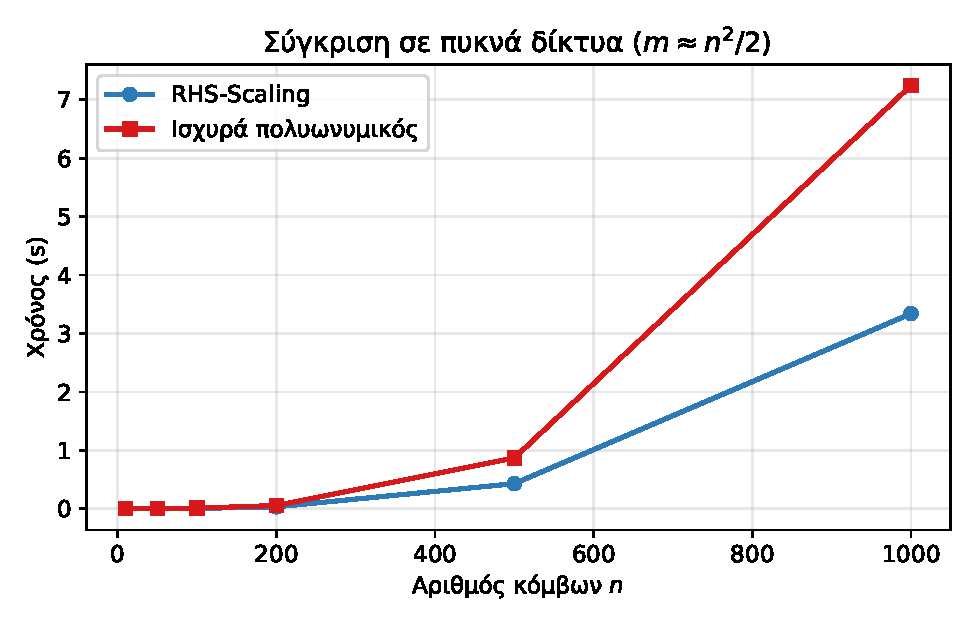
\includegraphics[width=0.85\textwidth]{media/diagram_4_1_size_dense.pdf}
\caption{Χρόνοι εκτέλεσης σε πυκνά δίκτυα ως συνάρτηση του $n$.}
\label{fig:size-dense}
\end{figure}

\begin{table}[h]
\centering
\caption{Χρόνοι εκτέλεσης σε αραιά δίκτυα, $m \approx 3n$ (μέσος όρος 5 εκτελέσεων).}
\label{tab:sparse}
\begin{tabular}{rrcc}
\toprule
$n$ & $m$ & \textenglish{RHS-Scaling} & Ισχυρά πολυωνυμικός \\
\midrule
  50 & 150 & 1.06\,ms & 1.22\,ms \\
  100 & 300 & 1.28\,ms & 1.48\,ms \\
  200 & 600 & 2.29\,ms & 2.94\,ms \\
  500 & 1500 & 8.02\,ms & 13.59\,ms \\
  1000 & 3000 & 26.75\,ms & 44.00\,ms \\
\bottomrule
\end{tabular}
\end{table}


\begin{figure}[h]
\centering
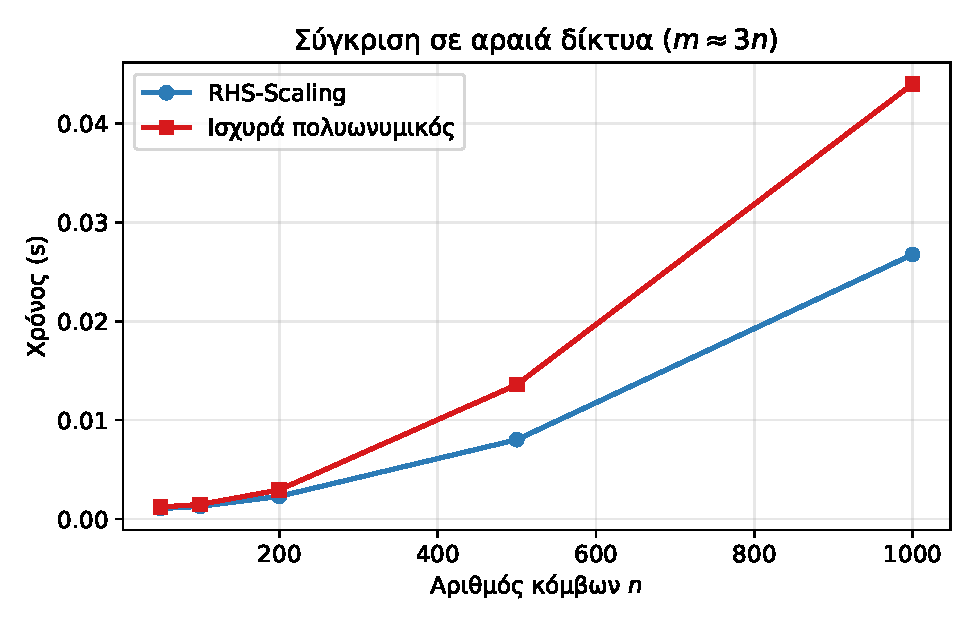
\includegraphics[width=0.85\textwidth]{media/diagram_4_2_size_sparse.pdf}
\caption{Χρόνοι εκτέλεσης σε αραιά δίκτυα ($m \approx 3n$).}
\label{fig:size-sparse}
\end{figure}

Και στα δύο σενάρια ο \textenglish{RHS-Scaling} είναι ταχύτερος για μικρές τιμές $U$. Στα πυκνά δίκτυα ο λόγος χρόνων αυξάνεται σταδιακά με το $n$, φτάνοντας ${\sim}2.1$ για $n = 1000$. Στα αραιά ο λόγος κυμαίνεται στο ${\sim}1.6$ για $n = 1000$. Η διαφορά στους απόλυτους χρόνους είναι μεγάλη: για $n = 1000$ τα πυκνά δίκτυα χρειάζονται ${\sim}3.3$\,s (\textenglish{RHS-Scaling}) ενώ τα αραιά μόλις ${\sim}25$\,ms, αφού η υλοποίηση \textenglish{Dijkstra} σαρώνει $m$ ακμές ανά γύρο και η πολυπλοκότητα ανά κλήση είναι $O(nm)$.

\subsection{Επίδραση του αριθμού πηγών και καταβοθρών}

Στο δεύτερο πείραμα διατηρείται σταθερό μέγεθος $n = 500$ και μεταβάλλεται ο αριθμός πηγών και καταβοθρών ($n_{\text{src}} = n_{\text{sink}}$) από 1 έως 20, με συνολική προσφορά 100.

\begin{table}[h]
\centering
\caption{Πηγές/καταβόθρες σε πυκνά δίκτυα ($n = 500$, μέσος όρος 5 εκτελέσεων).}
\label{tab:sources-dense}
\begin{tabular}{rcc}
\toprule
$n_{\text{src}} = n_{\text{sink}}$ & \textenglish{RHS-Scaling} & Ισχυρά πολυωνυμικός \\
\midrule
  1 & 426.37\,ms & 870.01\,ms \\
  2 & 927.92\,ms & 1.598\,s \\
  5 & 1.605\,s & 3.212\,s \\
  10 & 2.633\,s & 5.553\,s \\
  20 & 3.993\,s & 8.804\,s \\
\bottomrule
\end{tabular}
\end{table}


\begin{figure}[h]
\centering
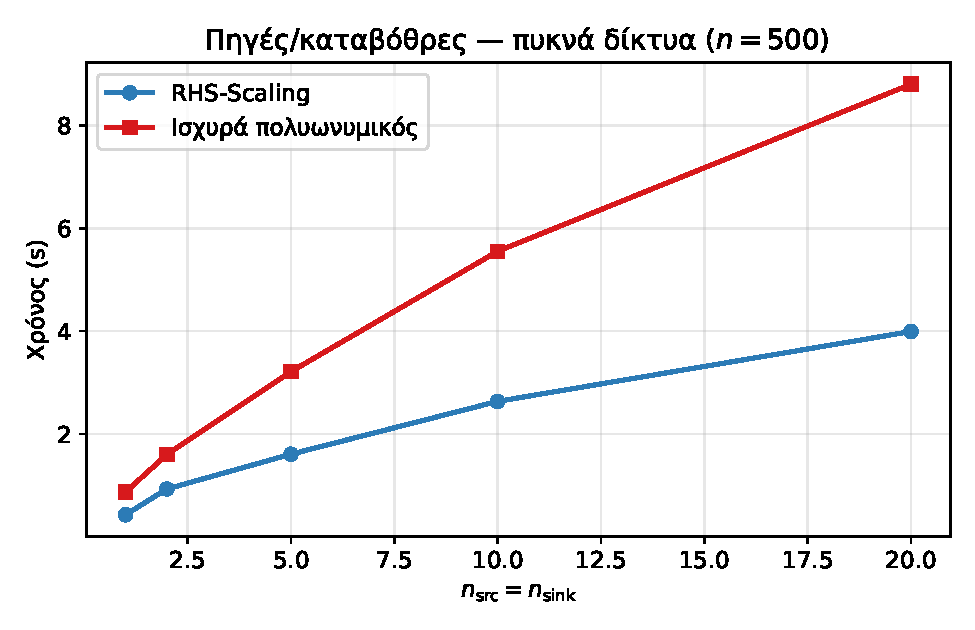
\includegraphics[width=0.85\textwidth]{media/diagram_4_3_sources_dense.pdf}
\caption{Επίδραση πηγών/καταβοθρών σε πυκνά δίκτυα ($n = 500$).}
\label{fig:sources-dense}
\end{figure}

\begin{table}[h]
\centering
\caption{Πηγές/καταβόθρες σε αραιά δίκτυα ($n = 500$, $m \approx 3n$, μέσος όρος 5 εκτελέσεων).}
\label{tab:sources-sparse}
\begin{tabular}{rcc}
\toprule
$n_{\text{src}} = n_{\text{sink}}$ & \textenglish{RHS-Scaling} & Ισχυρά πολυωνυμικός \\
\midrule
  1 & 7.47\,ms & 13.71\,ms \\
  2 & 17.94\,ms & 25.69\,ms \\
  5 & 25.84\,ms & 48.42\,ms \\
  10 & 36.35\,ms & 68.45\,ms \\
  20 & 56.26\,ms & 117.87\,ms \\
\bottomrule
\end{tabular}
\end{table}


\begin{figure}[h]
\centering
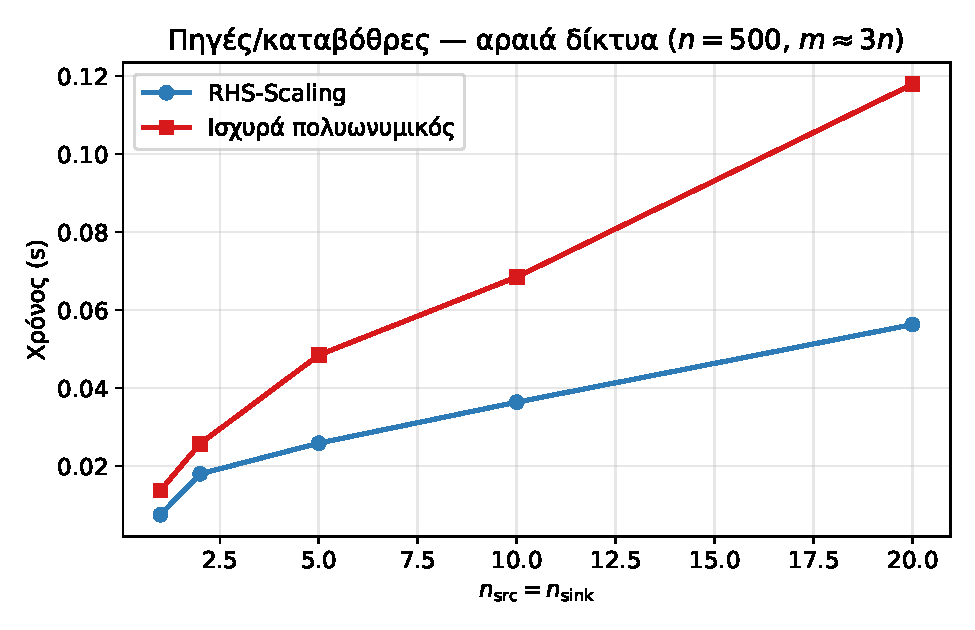
\includegraphics[width=0.85\textwidth]{media/diagram_4_4_sources_sparse.pdf}
\caption{Επίδραση πηγών/καταβοθρών σε αραιά δίκτυα ($n = 500$, $m \approx 3n$).}
\label{fig:sources-sparse}
\end{figure}

Περισσότερες πηγές και καταβόθρες σημαίνει περισσότερους κόμβους που πρέπει να ισορροπηθούν σε κάθε $\Delta$-φάση, άρα περισσότερες επαυξήσεις. Αυτό φαίνεται καθαρά στα δεδομένα: με $k = 20$ ο χρόνος αυξάνεται κατά ${\sim}10\times$ στα πυκνά και κατά ${\sim}8\times$ στα αραιά σε σχέση με $k = 1$. Ο λόγος χρόνων μεταξύ των δύο αλγορίθμων παραμένει σχετικά σταθερός (${\sim}2\times$ στα πυκνά, ${\sim}1.8\times$ στα αραιά), ανεξάρτητα από τον αριθμό πηγών/καταβοθρών.

\subsection{Επίδραση του εύρους τιμών προσφοράς/ζήτησης}

Στο τρίτο πείραμα διατηρούνται σταθεροί $n = 500$ κόμβοι και 5 πηγές/καταβόθρες, ενώ μεταβάλλεται η συνολική προσφορά $U \in \{100,\, 10^3,\, 10^4,\, 10^5,\, 10^6\}$, χωρίς αλλαγή στην τοπολογία. Τα αποτελέσματα παρουσιάζονται στο Σχήμα~\ref{fig:supply-dense} (πυκνά) και στο Σχήμα~\ref{fig:supply-sparse} (αραιά).

\begin{figure}[h]
\centering
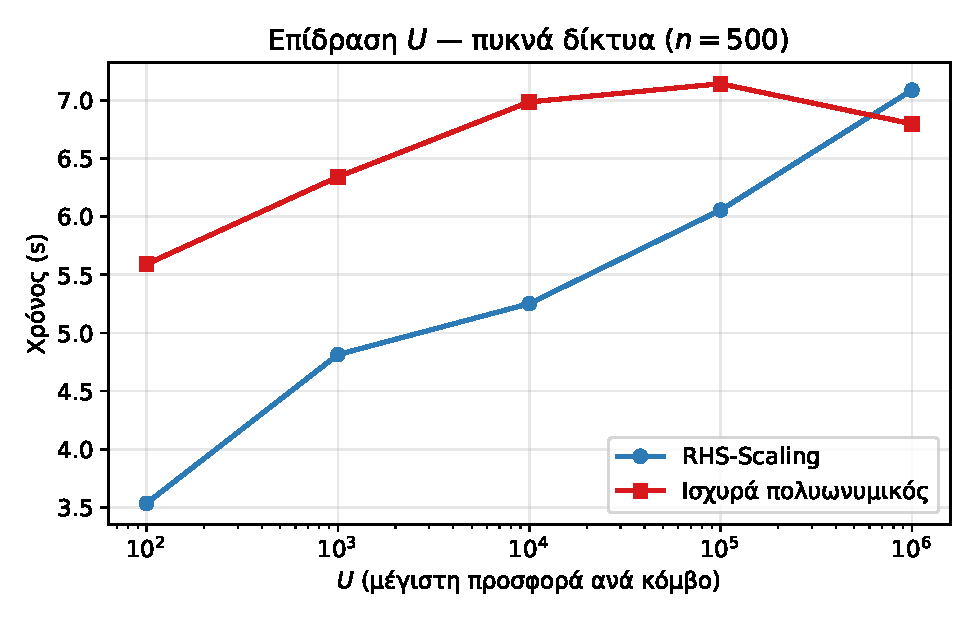
\includegraphics[width=0.85\textwidth]{media/diagram_4_5_supply_dense.pdf}
\caption{Χρόνοι εκτέλεσης ως συνάρτηση του $U$ σε πυκνά δίκτυα ($n = 500$).}
\label{fig:supply-dense}
\end{figure}

\begin{figure}[h]
\centering
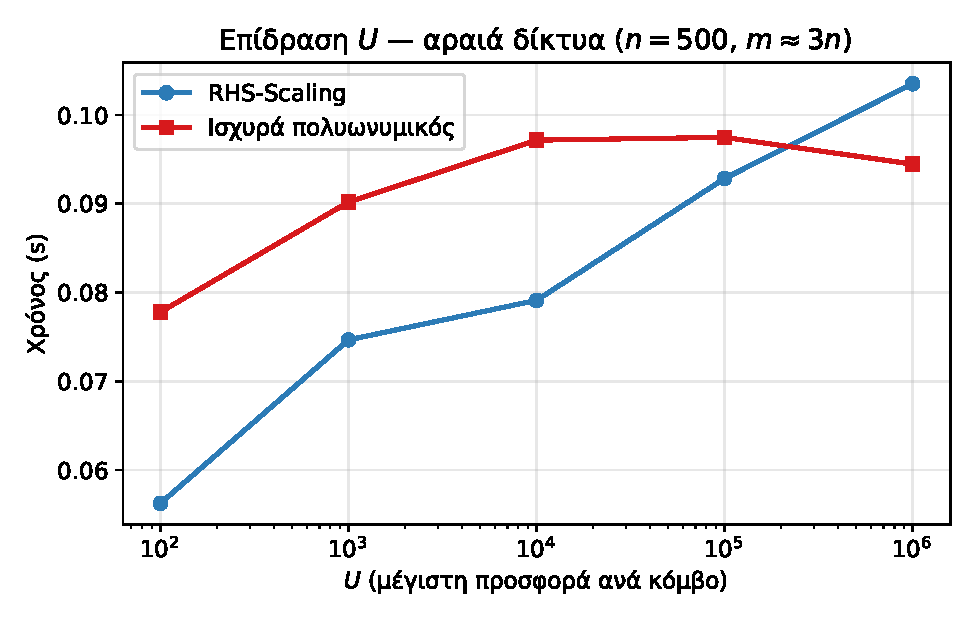
\includegraphics[width=0.85\textwidth]{media/diagram_4_6_supply_sparse.pdf}
\caption{Χρόνοι εκτέλεσης ως συνάρτηση του $U$ σε αραιά δίκτυα ($n = 500$, $m \approx 3n$).}
\label{fig:supply-sparse}
\end{figure}

Ο \textenglish{RHS-Scaling} δείχνει μονοτονική αύξηση με το $U$, σύμφωνα με τον παράγοντα $\log U$ στην πολυπλοκότητά του. Ο ισχυρά πολυωνυμικός αλγόριθμος αυξάνεται αρχικά αλλά για $U = 10^6$ ο χρόνος του σταθεροποιείται ή μειώνεται, χάρη στη σύμπτυξη ακμών που μειώνει το ενεργό μέγεθος του γραφήματος. Στο $U = 10^6$ ο ισχυρά πολυωνυμικός γίνεται ταχύτερος τόσο στα πυκνά όσο και στα αραιά δίκτυα. Αυτό το αποτέλεσμα συμφωνεί με τη θεωρητική ανάλυση: για αρκετά μεγάλο $U$ ο παράγοντας $\log n$ του ισχυρά πολυωνυμικού υπερτερεί του $\log U$ του \textenglish{RHS-Scaling}.

\section{Σύνοψη πειραματικών αποτελεσμάτων}

Από τα πειράματα αυτού του κεφαλαίου προκύπτουν τρία συμπεράσματα. Πρώτον, και οι δύο υλοποιήσεις παράγουν βέλτιστο κόστος ταυτόσημο με αυτό της \textenglish{NetworkX} σε κάθε περίπτωση που δοκιμάστηκε. Δεύτερον, για μικρές τιμές $U$ ο \textenglish{RHS-Scaling} είναι ταχύτερος, καθώς η επιβάρυνση που εισάγουν οι μηχανισμοί σύμπτυξης, αναίρεσης και τελικής μέγιστης ροής δεν αντισταθμίζεται από τη μείωση φάσεων. Τρίτον, καθώς αυξάνεται το $U$ ο ισχυρά πολυωνυμικός γίνεται ταχύτερος (στο $U = 10^6$), τόσο σε πυκνά όσο και σε αραιά δίκτυα, σε συμφωνία με τη θεωρητική ανάλυση.

\chapter{Συμπεράσματα}

\section{Συμπεράσματα}

Η παρούσα εργασία παρουσίασε τη θεωρητική ανάλυση και τη λεπτομερή υλοποίηση του αλγορίθμου ροής ελαχίστου κόστους του \textenglish{James~B.~Orlin} (1993). Υλοποιήθηκαν δύο εκδοχές σε γλώσσα \textenglish{C}: η τεχνική κλιμάκωσης των \textenglish{Edmonds-Karp} (\textenglish{Section~3} του άρθρου) και ο πλήρης ισχυρά πολυωνυμικός αλγόριθμος με συμπτύξεις (\textenglish{Section~4}).

Η υλοποίηση ανέδειξε τις λεπτομέρειες στον χειρισμό των συμπτύξεων και των δυναμικών. Ιδιαίτερα οι μηχανισμοί πλήρους αναγέννησης του $\Delta$, η αναίρεση συμπτύξεων με αποκατάσταση δυναμικών, και ο τελικός υπολογισμός βέλτιστης ροής μέσω μέγιστης ροής, απαιτούν προσεκτικό συντονισμό και αποθήκευση επαρκών στιγμιοτύπων κατάστασης.

Η χρήση της γεννήτριας σε \textenglish{Python} με τη \textenglish{NetworkX} ως αναφορά ορθότητας αποδείχθηκε χρήσιμη: επιτρέπει τον έλεγχο πολλαπλών δικτύων με διαφορετικές παραμέτρους και αποκαλύπτει ενδεχόμενα σφάλματα στην υλοποίηση. Η μέτρηση χρόνων εκτέλεσης επιβεβαιώνει την πρακτική υπεροχή του απλού \textenglish{RHS-Scaling} για μικρές τιμές $U$, αλλά αναδεικνύει και τη σημασία του ισχυρά πολυωνυμικού αλγορίθμου όταν το $U$ γίνει εξαιρετικά μεγάλο.

\section{Μελλοντικές επεκτάσεις}

Πιθανές επεκτάσεις περιλαμβάνουν τις εξής. Πρώτον, η αντικατάσταση της γραμμικής υλοποίησης του \textenglish{Dijkstra} με μια υλοποίηση που βασίζεται σε \textenglish{binary heap} ή σε \textenglish{Fibonacci heap} θα βελτιώσει τον χρόνο ανά συντομότερο μονοπάτι και θα φέρει την πρακτική συμπεριφορά πιο κοντά στο θεωρητικό βέλτιστο.

Δεύτερον, η υποστήριξη χωρητικών δικτύων, είτε εσωτερικά στον κώδικα είτε μέσω εξωτερικού μετασχηματισμού που διαχωρίζει κάθε χωρητική ακμή σε νέο κόμβο και δύο μη χωρητικές ακμές, θα διευρύνει το εύρος εφαρμογών. Η υλοποίηση μπορεί να επεκταθεί ώστε να αποδεχθεί και αρχεία εισόδου με χωρητικότητες.

Τρίτον, η βελτίωση της γεννήτριας δοκιμών, ώστε να παράγει δίκτυα με καθορισμένη δομή (π.χ.\ \textenglish{bipartite matching}, \textenglish{transportation problems}, \textenglish{planar networks}), θα επιτρέψει πιο στοχευμένη πειραματική αξιολόγηση. Επίσης, μια πιθανή επέκταση είναι η σύγκριση των αποτελεσμάτων με άλλους αλγορίθμους (π.χ.\ \textenglish{Network Simplex}, \textenglish{Cost-Scaling}), που διαφορετικά βασίζονται στο ίδιο θεωρητικό υπόβαθρο.

Τέλος, το άρθρο του \textenglish{Orlin} αναφέρει ότι ο αλγόριθμος μπορεί να υλοποιηθεί παράλληλα σε χρόνο $O(m \log^3 n)$ με $O(n^3)$ επεξεργαστές. Μια μελλοντική εργασία θα μπορούσε να εξετάσει εμπειρικά την παραλληλοποίηση του \textenglish{Dijkstra} στο εσωτερικό του αλγορίθμου.

% =============== ΒΙΒΛΙΟΓΡΑΦΙΑ ===============

\begin{thebibliography}{99}
\addcontentsline{toc}{chapter}{Βιβλιογραφία}
\small

\bibitem{orlin1993}
Orlin, J.~B. (1993). A Faster Strongly Polynomial Minimum Cost Flow Algorithm. \textit{Operations Research}, 41(2), 338--350.

\bibitem{edmondskarp1972}
Edmonds, J., \& Karp, R.~M. (1972). Theoretical Improvements in Algorithmic Efficiency for Network Flow Problems. \textit{Journal of the ACM}, 19, 248--264.

\bibitem{tardos1985}
Tardos, É. (1985). A Strongly Polynomial Minimum Cost Circulation Algorithm. \textit{Combinatorica}, 5, 247--255.

\bibitem{galiltardos1986}
Galil, Z., \& Tardos, É. (1986). An $O(n^2 (m + n \log n) \log n)$ Min-Cost Flow Algorithm. In \textit{Proceedings of the 27th Annual Symposium on Foundations of Computer Science}, 136--146.

\bibitem{goldbergtarjan1987}
Goldberg, A.~V., \& Tarjan, R.~E. (1987). Solving Minimum Cost Flow Problems by Successive Approximation. In \textit{Proceedings of the 19th ACM Symposium on the Theory of Computing}, 7--18.

\bibitem{goldbergtarjan1988}
Goldberg, A.~V., \& Tarjan, R.~E. (1988). Finding Minimum-Cost Circulations by Canceling Negative Cycles. In \textit{Proceedings of the 20th ACM Symposium on the Theory of Computing}, 388--397.

\bibitem{ahujadoublescaling}
Ahuja, R.~K., Goldberg, A.~V., Orlin, J.~B., \& Tarjan, R.~E. (1988). Finding Minimum Cost Flows by Double Scaling. \textit{Mathematical Programming}, 53, 243--266.

\bibitem{ahujabook}
Ahuja, R.~K., Magnanti, T.~L., \& Orlin, J.~B. (1993). \textit{Network Flows: Theory, Algorithms, and Applications}. Prentice Hall, Englewood Cliffs, NJ.

\bibitem{fredmantarjan1987}
Fredman, M.~L., \& Tarjan, R.~E. (1987). Fibonacci Heaps and Their Uses in Improved Network Optimization Algorithms. \textit{Journal of the ACM}, 34, 596--615.

\bibitem{dijkstra1959}
Dijkstra, E.~W. (1959). A Note on Two Problems in Connexion with Graphs. \textit{Numerische Mathematik}, 1, 269--271.

\bibitem{fujishige1986}
Fujishige, S. (1986). An $O(m^3 \log n)$ Capacity-Rounding Algorithm for the Minimum Cost Circulation Problem: A Dual Framework of Tardos' Algorithm. \textit{Mathematical Programming}, 35, 298--309.

\bibitem{rock1980}
Röck, H. (1980). Scaling Techniques for Minimal Cost Network Flows. In \textit{Discrete Structures and Algorithms}, Carl Hansen, Munich, 101--191.

\bibitem{fordfulkerson}
Ford, L.~R., Jr., \& Fulkerson, D.~R. (1962). \textit{Flows in Networks}. Princeton University Press.

\bibitem{networkx}
NetworkX Developers. NetworkX: Network analysis in Python. \url{https://networkx.org/}

\bibitem{hagberg2008}
Hagberg, A.~A., Schult, D.~A., \& Swart, P.~J. (2008). Exploring Network Structure, Dynamics, and Function using NetworkX. In \textit{Proceedings of the 7th Python in Science Conference (SciPy2008)}, 11--15.

\end{thebibliography}

% =============== ΠΑΡΑΡΤΗΜΑ ===============

\appendix
\chapter{Μετάφραση ξένων όρων}

Ο παρακάτω πίνακας συνοψίζει τους κυριότερους ξένους όρους που χρησιμοποιούνται στην εργασία και τις ελληνικές αποδόσεις τους.

\begin{center}
\small
\renewcommand{\arraystretch}{1.2}
\begin{tabularx}{\linewidth}{@{}>{\raggedright\arraybackslash}X >{\raggedright\arraybackslash\itshape}X@{}}
\toprule
\textbf{Ελληνικός όρος} & \textbf{\textup{Ξένος όρος (Αγγλικός)}} \\
\midrule
Ροή ελαχίστου κόστους & \textenglish{Minimum cost flow} \\
Δίκτυο ροής & \textenglish{Flow network} \\
Ψευδοροή & \textenglish{Pseudoflow} \\
Υπολειπόμενο δίκτυο & \textenglish{Residual network} \\
Μειωμένο κόστος & \textenglish{Reduced cost} \\
Δυναμικό κόμβου & \textenglish{Node potential} \\
Κλιμάκωση δεξιού μέλους & \textenglish{Right-hand side scaling} \\
Ισχυρά πολυωνυμικός αλγόριθμος & \textenglish{Strongly polynomial algorithm} \\
Ισχυρά εφικτή ακμή & \textenglish{Strongly feasible arc} \\
Σύμπτυξη κόμβων & \textenglish{Node contraction} \\
Αναίρεση σύμπτυξης & \textenglish{Uncontraction} \\
Πλήρης αναγέννηση & \textenglish{Complete regeneration} \\
Φάση κλιμάκωσης & \textenglish{Scaling phase} \\
Συντομότερο μονοπάτι & \textenglish{Shortest path} \\
Επαύξηση ροής & \textenglish{Flow augmentation} \\
Ισορροπία μάζας & \textenglish{Mass balance} \\
Πλεόνασμα / Υπερβάλλον & \textenglish{Excess / Imbalance} \\
Πηγή / Καταβόθρα & \textenglish{Source / Sink} \\
Μέγιστη ροή & \textenglish{Maximum flow} \\
Ισχυρά συνδεδεμένο γράφημα & \textenglish{Strongly connected graph} \\
Χωρητικότητα & \textenglish{Capacity} \\
Κόστος ακμής & \textenglish{Arc cost} \\
Υπερ-πηγή / Υπερ-καταβόθρα & \textenglish{Super source / Super sink} \\
Συνθήκη συμπληρωματικής χαλαρότητας & \textenglish{Complementary slackness condition} \\
Τεχνική διπλής κλιμάκωσης & \textenglish{Double scaling technique} \\
\bottomrule
\end{tabularx}
\end{center}

\end{document}
